%%%%%%%%%%%%%%%%%%%%%%% file template.tex %%%%%%%%%%%%%%%%%%%%%%%%%
\RequirePackage{fix-cm}
\documentclass[smallextended]{svjour3}
\smartqed
\usepackage{graphicx}
\usepackage{natbib}
\usepackage{url}
\usepackage{float}
\usepackage{placeins}
\usepackage{multirow}
\usepackage{array,tabularx}


\usepackage{xcolor}
\usepackage{listings}

\lstdefinestyle{ccscode}{
  basicstyle=\ttfamily\footnotesize,
  backgroundcolor=\color{gray!5},
  frame=single,
  rulecolor=\color{gray!50},
  framerule=0.4pt,
  framesep=6pt,
  numbers=none,
  columns=fullflexible,
  keepspaces=true,
  showstringspaces=false,
  breaklines=true,
  moredelim=**[is][\color{green!50!black}]{|+|}{|/|}
}


\newcolumntype{Y}{>{\raggedright\arraybackslash}X}
\usepackage{amsmath}
\usepackage[colorlinks=true,citecolor=black,linkcolor=blue,urlcolor=blue]{hyperref}
\bibpunct{(}{)}{;}{a}{\ }{;}
\makeatletter
\renewcommand{\hyper@natlinkbreak}[2]{%
  \hyper@natlinkend#1\hyper@linkstart{cite}{cite.#2}\color{blue}}
% Unnumbered, stand-alone headings for the dataset-construction steps.
\newcommand{\datastepheading}{%
  \@startsection{paragraph}{4}{\z@}{-8pt}{3pt}%
    {\normalfont\normalsize\bfseries}*}
\makeatother
\setlength{\tabcolsep}{3pt}
\setlength{\emergencystretch}{3em}
\newcommand{\rqanswer}[2]{%
\begin{center}
\fbox{\begin{minipage}{0.94\linewidth}
\small\textbf{Answer to #1.} #2
\end{minipage}}
\end{center}}
\journalname{Empirical Software Engineering}

\begin{document}

\title{Cache Configuration Smells in GitHub Actions: A Large-Scale Empirical Study}
\titlerunning{CCS in GitHub Actions}

% ================= Authors =================
\author{
    Siyu Wang \and
    Yang Zhang \and
    Changrong Xie \and
    Jiacheng Jie \and
    Youren Chen \and
    Zezhou Tang \and
    Tanghaoran Zhang \and
    Xinjun Mao
}
\authorrunning{Siyu Wang et al.}

% ================= Affiliation =================
\institute{
    Siyu Wang, Yang Zhang, Changrong Xie, Jiacheng Jie,
    Youren Chen, Zezhou Tang, Tanghaoran Zhang, Xinjun Mao
    \at
    College of Computer Science and Technology, National University of Defense and Technology,
    Changsha, China \\
    \\
    \textbf{Corresponding author:} Xinjun Mao \\
    \email{xjmao@nudt.edu.cn}
}

\date{}

\maketitle

\begin{abstract}
Long continuous integration runs delay developer feedback and increase computing costs. Caching helps reduce repeated work, but its benefits depend on appropriate configuration. We refer to recurring configuration patterns that may hinder cache reuse or maintenance as cache configuration smells (CCS). Although previous studies have investigated caching practices, little is known about how widespread CCS are in GitHub Actions and how they relate to workflow outcomes. In this paper, we characterize 11 CCS types and develop a static detector to identify them in workflow configurations. We conduct a large-scale empirical study of 118,402 workflows from 19,324 public repositories and more than one million workflow runs. Our results show that 22.29\% of workflows contain at least one detected CCS, spanning 54.48\% of the studied repositories. Missing dependency caching is the most common CCS type. We identify four CCS types significantly associated with longer completed runs, with adjusted duration ratios corresponding to 12.3\%--74.7\% longer duration. Missing dependency caching, missing fallback matching, and deprecated cache actions are significantly associated with lower workflow-run success probability. Separate descriptive comparisons reveal differences in runner time and estimated runner costs. These findings highlight cache configuration as an important consideration in workflow efficiency and provide empirical guidance for configuration review and cache-aware tool development.


\keywords{GitHub Actions \and CI/CD \and CCS \and Caching \and Workflow Outcomes}
\end{abstract}

\section{Introduction}
\label{sec:intro}

Continuous Integration and Continuous Deployment (CI/CD) automate software integration, testing, and release to shorten feedback cycles and reduce integration risk~\citep{duvall2007continuous,shahin2017continuous}. Empirical studies relate CI duration and breakages to project, configuration, and execution characteristics~\citep{ghaleb2019empirical,ghaleb2022studying}. Industrial systems such as CloudBuild combine content-based caching with parallel execution to shorten build and test cycles~\citep{esfahani2016cloudbuild}. For GitHub Actions, resource-use analysis identifies testing and building as major consumers and caching as an underused optimization opportunity~\citep{bouzenia2024resource}. However, an empirical study of Travis CI shows that caching does not consistently reduce build duration and requires ongoing maintenance~\citep{ghaleb2026cachingreality}. These findings motivate examining how caches are configured and maintained, beyond whether caching is enabled. In GitHub Actions, cache paths, keys, fallback matching, and step order shape whether cached content can be reused effectively~\citep{hasan2026caching,gha_cache_docs}.

GitHub Actions is widely used for CI/CD across public software repositories~\citep{decan2022use}. It provides several ways to configure caching, including explicit cache actions, language setup actions with built-in package-manager caches, and Docker-layer caches~\citep{hasan2026caching,gha_cache_docs}. These mechanisms expose configuration choices involving cache paths, keys, fallback options, and action-specific inputs~\citep{hasan2026caching,gha_cache_docs}.

Recent studies have examined CI/CD caching practices, configuration problems, and execution outcomes. \citet{hasan2026caching} study how developers adopt, use, and evolve caching in GitHub Actions, with an emphasis on configuration practices and maintenance. \citet{ghaleb2026cachingreality} investigate caching adoption and maintenance in Travis CI, together with changes in build duration and the overhead of cache operations. \citet{urdih2026cache} present a catalog of cache-related smells in GitLab CI/CD based on official documentation and practitioner-oriented grey literature. They develop a static detector and evaluate its detection accuracy and the prevalence of the detected smells. Although they also discuss the applicability of several smells to GitHub Actions, their empirical evaluation focuses on GitLab. Thus, evidence remains limited on the prevalence of cache configuration smells (CCS) in GitHub Actions and their associations with workflow execution outcomes. To address this gap, we define static detection rules for CCS in GitHub Actions and conduct an empirical study of their occurrence patterns. We further examine associations between individual CCS types and workflow-run duration and success.

Following prior configuration-smell research~\citep{sharma2016configuration,vassallo2020cd,gallaba2020travis,zhang2022buildsonic,khatami2024gha}, we treat CCS as a recurring cache-configuration pattern that can be statically recognized as potentially harmful, while separating static evidence from runtime effects.

Building on this definition, we implement and validate static detection rules for 11 CCS types in GitHub Actions. Throughout the research questions, CCS denotes these 11 operationalized patterns identified by static YAML rules. We organize the study around two research questions and their subquestions:

\begin{itemize}
  \item \textbf{RQ1 (Prevalence and Occurrence Patterns):} How widespread are CCS in GitHub Actions workflows, and what patterns characterize their occurrence?
  \begin{itemize}
    \item \textbf{RQ1.1 (Prevalence and Context):} How prevalent are individual CCS types across workflows and repositories, and how are they distributed across workflow and repository contexts?
    \item \textbf{RQ1.2 (Multiplicity and Co-occurrence):} How often do multiple CCS occur within a workflow, and which types tend to co-occur?
  \end{itemize}

  \item \textbf{RQ2 (Duration, Success, and Resource Use):} How do CCS relate to workflow-run duration and success, and to runner resource use?
  \begin{itemize}
    \item \textbf{RQ2.1 (Duration):} How is each CCS type associated with the duration of completed workflow runs?
    \item \textbf{RQ2.2 (Success):} How is each CCS type associated with workflow-run success?
    \item \textbf{RQ2.3 (Exploratory Resource Use):} How do runner-allocated VM time and cost differ between workflows with and without each CCS type?
  \end{itemize}

\end{itemize}

Our main contributions are as follows:
\begin{enumerate}
  \item \textbf{CCS Operationalization and Detection:} We operationalize 11 CCS types as reproducible, GitHub Actions-specific YAML rules by triangulating platform documentation, prior work, workflow configurations, and revision cases. We evaluate the detector on 383 manually annotated workflows.

  \item \textbf{Large-Scale Empirical Characterization:} We quantify prevalence, co-occurrence, and contextual distribution in 118,402 parseable workflows from 19,324 repositories. We then use 1,091,978 detector-valid, version-aligned runs from 51,097 workflow versions in 14,695 repositories to estimate adjusted associations with completed-run duration and success. Four CCS types were associated with longer duration and three with lower success probability after BH adjustment. A separate historical extension covers 166 configuration changes and 1,268 successful runs, comparing runner-allocated VM time and estimated runner cost within workflows.
\end{enumerate}

The detector, workflow annotations, coding records, analysis scripts, and result artifacts will be made available in a versioned replication package at \url{https://github.com/ilikefish233/gha_log_analysis}.

The remainder is organized as follows. Section~\ref{sec:background} presents GitHub Actions caching. Section~\ref{sec:related_work} reviews prior work, and Section~\ref{sec:methodology} describes the study design, CCS operationalization, detector, and analyses. Section~\ref{sec:results} reports the findings, Section~\ref{sec:discussion} discusses implications, and Section~\ref{sec:threats} addresses validity threats before the conclusion in Section~\ref{sec:conclusion}.

\section{Background: Caching in GitHub Actions}
\label{sec:background}

This section introduces the GitHub Actions caching mechanisms and execution semantics needed to interpret CCS. We first distinguish the three main caching mechanisms identified in prior work, then describe cache restoration, matching, and saving, and finally explain how execution order and job relationships shape cache behavior.

\subsection{Caching Mechanisms in GitHub Actions}

GitHub Actions workflows are defined in YAML as one or more jobs, each composed of an ordered sequence of steps~\citep{gha_workflow_docs}. Prior work distinguishes three main caching mechanisms in GitHub Actions workflows~\citep{hasan2026caching}. First, explicit caching uses \texttt{actions/cache}, for which developers specify cache paths and keys. Second, package-manager caching is enabled through cache-related inputs of language or tool setup actions, such as \texttt{setup-node} and \texttt{setup-python}~\citep{gha_cache_docs}. Third, Docker layer caching is configured through Docker build tooling to reuse previously built image layers~\citep{hasan2026caching}. Because these mechanisms encode caching through different actions and inputs, identifying cache use requires more than searching for \texttt{actions/cache} steps.

\enlargethispage{3\baselineskip}
\subsection{Cache Lifecycle and Matching}

For explicit cache actions, \texttt{path} specifies the files, directories, or glob patterns to cache and restore, whereas \texttt{key} provides the primary lookup key~\citep{gha_cache_docs}. Cache lookup is additionally constrained by a computed cache version and the ref scope associated with the workflow run. GitHub first searches the accessible cache scope using the primary key and then evaluates any declared \texttt{restore-keys} in order. When multiple caches match a fallback prefix, the most recently created entry is selected~\citep{gha_cache_docs}. If no matching entry is found in the current ref scope, the search is repeated in the default-branch scope. Pull-request runs may additionally access caches from their base branch, subject to GitHub's cache-access restrictions~\citep{gha_cache_docs}. The cache version is derived from the cached paths and compression method, so entries with the same textual key but different versions are treated as distinct caches~\citep{gha_cache_docs}. Because fallback reuse may be inappropriate or unnecessary for some cached resources, this study does not treat the absence of \texttt{restore-keys} alone as a CCS finding. The corresponding eligibility conditions are defined in Section~\ref{sec:methodology}.

Restoration and saving form a lifecycle rather than a single lookup. The combined \texttt{actions/cache} action restores an available entry when its step runs. After a miss or partial match, later steps may consume or populate the path, and a new entry for the primary key is created only if the job succeeds~\citep{gha_cache_docs}. The \texttt{actions/cache/restore} and \texttt{actions/cache/save} variants separate these phases, permitting an explicit save after the producer while restoration still precedes the consumer~\citep{gha_cache_strategies}. Thus, the relevant sequence is restore, consumer or producer execution, and post-job or explicit save.

Existing entries are immutable, so changed content requires a new key~\citep{gha_cache_docs}. A run-specific key may therefore be intentional when each run creates a fresh entry, while a broader restore-key prefix may permit reuse of an earlier compatible cache~\citep{gha_cache_tips}. These constraints inform whether a write is reachable, a cache step precedes its intended producer or consumer, and repeated updates can create reusable entries.

\subsection{Execution Context and Cross-Job Semantics}

Cache behavior further depends on execution order. A key derived from repository files requires those files before \texttt{hashFiles} is evaluated, whereas an independent key may not require checkout first. Restoring a dependency cache after installation cannot benefit that installation, but later restoration may be appropriate when a subsequent step consumes the content~\citep{gha_cache_docs}. Ordering should therefore be interpreted in relation to the cache's intended consumer rather than judged from position alone.

After simultaneous misses, parallel jobs may independently prepare equivalent content and attempt to save the same key. Because entries are immutable, this can duplicate preparation or produce competing save attempts~\citep{gha_cache_docs}.\footnote{A related developer report discusses duplicate cache entries under high concurrency: \url{https://github.com/actions/cache/issues/1392}.} Concurrent use is not inherently defective. Interpretation depends on whether jobs intentionally produce distinct content and whether their dependencies coordinate population and reuse.

Caches and workflow artifacts serve different purposes. A cache accelerates reuse of files across runs, and a job should be able to download or regenerate them when no cache is available. An artifact preserves output from a particular run for later inspection or transfers data between jobs in that run~\citep{gha_cache_concepts,gha_artifact_docs}. Treating cache availability as a correctness prerequisite therefore conflates reuse with durable output or inter-job transfer.

Together, these mechanisms show that cache configurations must be interpreted in context. The same syntax may be appropriate or problematic depending on the cached resource, matching strategy, execution order, and relationships among jobs. This semantic context provides the basis for the CCS definitions and detection rules introduced in Section~\ref{sec:methodology}.


\section{Related Work}
\label{sec:related_work}

\subsection{CI/CD Performance and Optimization}

Prior research has investigated factors affecting CI/CD performance and techniques for reducing build time and resource consumption. Ghaleb et al. examined factors associated with long CI builds and found that caching relatively stable content was associated with shorter build times~\citep{ghaleb2019empirical}. In a subsequent study, they investigated the relationship between build duration and build breakages, including the role of caching in build performance~\citep{ghaleb2022studying}. Gallaba et al. proposed Kotinos, which accelerates CI builds by inferring dependencies, caching build environments, and skipping unaffected build steps~\citep{gallaba2022caching}. Their evaluation showed that these techniques can substantially reduce build time without compromising build outcomes. Beyond caching, Jin and Servant compared CI improvement techniques and found that their benefits vary across measures of cost and feedback time~\citep{jin2021ci}.

Other studies have examined build performance and resource use in specific environments. Wu et al. investigated Docker build duration and developed prediction models using features of build contexts and configurations~\citep{wu2022dockerbuildduration}. For GitHub Actions, Bouzenia and Pradel analyzed workflow resource consumption and found that testing and building account for most of the resources used. They also identified opportunities to improve efficiency, including wider adoption of caching~\citep{bouzenia2024resource}. These findings provide context for studying cache configurations in relation to workflow duration and resource use.

\subsection{Configuration Smells in CI/CD}

Research on configuration smells has identified recurring configuration practices that may affect software maintenance and CI/CD execution. Sharma et al. developed a catalog of configuration smells in infrastructure code~\citep{sharma2016configuration}. Focusing on CI/CD, Zampetti et al. identified bad practices through developer interviews and Stack Overflow discussions~\citep{zampetti2020badpractices}. Vassallo et al. developed CI-Odor to detect CI process anti-patterns using build logs and repository information, and evaluated its reports through developer feedback~\citep{vassallo2019ciodor}.

Several studies have developed techniques for detecting configuration smells in CI/CD systems. CD-Linter detects configuration smells in GitLab CI/CD pipelines~\citep{vassallo2020cd}. Zhang et al. proposed BuildSonic, which identifies and repairs performance-related configuration smells in Travis CI, Maven, and Gradle configurations. Their evaluation also examined improvements in build performance after repairs~\citep{zhang2022buildsonic}. Gallaba et al. investigated the use and misuse of Travis CI features through HANSEL~\citep{gallaba2020travis}. For GitHub Actions, Khatami et al. identified potential workflow smells by analyzing recurring workflow changes and validated a subset through a contribution study~\citep{khatami2024gha}.

More closely related to caching, Urdih et al. developed a catalog of cache configuration smells for GitLab CI/CD and proposed CROSSER, a static detector for a subset of these smells~\citep{urdih2026cache}. They evaluated its detection accuracy and examined the prevalence of cache configuration smells in open-source projects. Their study provides empirical evidence of cache configuration problems in GitLab CI/CD. Our work examines these problems in GitHub Actions, whose caching mechanisms and configuration syntax require different detection rules, and relates the detected smells to workflow execution outcomes.

\subsection{GitHub Actions Practices and Evolution}

Studies of CI/CD adoption and evolution have examined how developers use and maintain workflow configurations. Decan et al. characterized the adoption of GitHub Actions in public repositories and the reuse of Actions across projects~\citep{decan2022use}. Zampetti et al. investigated CI/CD pipeline evolution and developed a taxonomy of restructuring activities based on changes to pipeline configurations~\citep{zampetti2021ci}. Decan et al. also examined outdated Action versions in GitHub Actions workflows, showing how reusable components may lag behind available releases~\citep{decan2023outdatedness}.

Other studies have investigated configuration challenges and workflow reliability. Zhang et al. analyzed problems reported by GitHub Actions developers on Stack Overflow and GitHub, along with the solutions discussed by practitioners~\citep{zhang2024ghaproblems}. Talebzadeh Bardsiri et al. examined the use of GitHub Actions language features and found that larger and more complex workflows are associated with higher failure rates and maintenance effort~\citep{bardsiri2026ghalanguage}.

Focusing specifically on caching, Hasan et al. investigated how developers adopt, configure, and evolve caching in GitHub Actions~\citep{hasan2026caching}. They found that caching is used across different job types and mechanisms, while cache configurations undergo frequent changes driven by maintenance needs. Cache configurations also have security implications, as improper cache isolation and reuse may expose workflows to cache poisoning attacks~\citep{cache_security_sp2024}.

Prior research has examined CI/CD performance, configuration smells, and caching practices across different platforms. Our study focuses on cache configuration smells in GitHub Actions, examining their prevalence and associations with workflow duration and success. We further compare runner time and estimated costs across historical versions of the same workflow with different detected CCS states.

\section{Methodology}
\label{sec:methodology}

\subsection{Designing the Study}

We examine the prevalence of cache configuration smells (CCS) in GitHub Actions and their associations with workflow execution outcomes. The definitions and detection rules follow GitHub Actions' cache behavior and workflow execution semantics. Their applicability to other CI/CD platforms requires further validation.

We define 11 CCS types based on prior research, platform documentation, and workflow cases, and implement static detection rules. We then collect workflow configurations and execution records, construct the datasets for RQ1 and RQ2, and evaluate the detector against manual annotations. RQ1 characterizes CCS prevalence, context, multiplicity, and co-occurrence. RQ2 examines associations with run duration and success, together with descriptive comparisons of runner time and estimated cost. Figure~\ref{fig:study-overview} summarizes the data sources, detection procedure, and analyses.

\begin{figure}
\centering
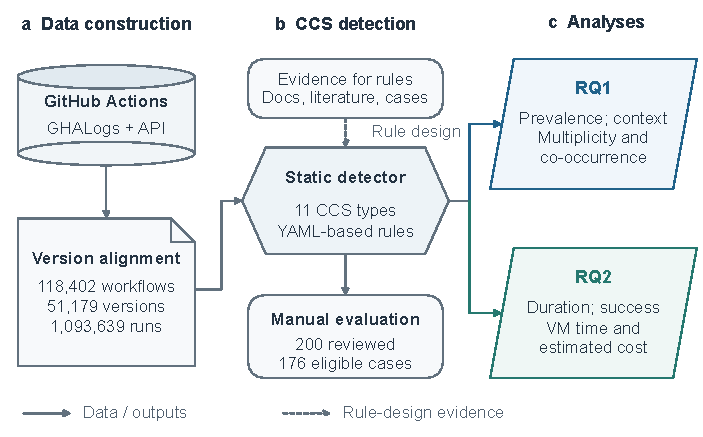
\includegraphics[width=\textwidth]{figures/Fig1.pdf}
\caption{Study overview:
\textbf{a} dataset construction;
\textbf{b} CCS rule design, detection, and evaluation;
\textbf{c} analyses addressing RQ1 and RQ2}
\label{fig:study-overview}
\end{figure}

% Local listing configuration: the pre-Methodology source is unchanged.
\lstdefinelanguage{CCSYAML}{
  sensitive=true,
  morecomment=[l]{\#},
  morestring=[b]',
  morestring=[b]",
  morekeywords={uses,with,run,jobs,steps,path,key,needs,cache,node-version,restore-keys,runs-on},
  keywordstyle=\color{blue!65!black}\bfseries,
  commentstyle=\color{green!35!black}\itshape,
  stringstyle=\color{orange!65!black}
}
\lstdefinestyle{ccside}{
  language=CCSYAML,
  basicstyle=\ttfamily\scriptsize,
  backgroundcolor=\color{gray!5},
  frame=single,rulecolor=\color{gray!45},framerule=0.4pt,
  framesep=5pt,numbers=left,numberstyle=\tiny\color{gray},
  numbersep=8pt,xleftmargin=15pt,xrightmargin=5pt,
  columns=fullflexible,keepspaces=true,showstringspaces=false,
  breaklines=true,breakatwhitespace=false,
  moredelim=**[is][\color{green!40!black}\bfseries]{|+|}{|/|}
}

\subsection{Cache Configuration Smells}
\label{sec:taxonomy}
\label{sec:smell-discovery}
\label{sec:case-evidence}

\lstdefinestyle{ccscase}{
  basicstyle=\ttfamily\fontsize{7.5}{9.0}\selectfont,
  backgroundcolor=\color{gray!4},
  frame=single,rulecolor=\color{gray!45},framerule=0.35pt,
  framesep=4pt,numbers=none,xleftmargin=4pt,xrightmargin=4pt,
  columns=fullflexible,keepspaces=true,showstringspaces=false,
  breaklines=true,breakatwhitespace=false,
  aboveskip=3pt,belowskip=4pt,
  moredelim=**[is][\color{blue!55!black}\bfseries]{|+|}{|/|}
}


We define CCS as recurring configuration patterns that may hinder cache reuse or maintenance. The catalog draws on related work, documented caching best practices, and workflow inspection supported by community discussions. We adapt four types from the GitLab CI/CD catalog: missing dependency caching, missing fallback matching, redundant cache updates, and missing Docker layer caching. These four smells are present in both GitLab CI/CD and GitHub Actions~\citep{urdih2026cache}. We also derive smells from violations of caching best practices documented by GitHub and Docker~\citep{gha_cache_docs,docker_gha_cache_docs}. We identify further smells through an extensive manual review of public GitHub Actions workflow configurations and corroborate them with evidence from developer discussions.

We focus on patterns that can be identified through static analysis of workflow configurations and group patterns describing the same problem under a single smell. For each smell, we design static detection rules based on GitHub Actions' caching policies and mechanisms, together with the characteristics of the smell itself. Table~\ref{tab:smell-catalog} summarizes the smells and their detection criteria. The following descriptions present the rationale, supporting evidence, detection conditions, and exceptions for each smell. 

\begin{table}[htbp]
\centering
\caption{Cache configuration smells and their detection criteria}
\label{tab:smell-catalog}
\scriptsize
\setlength{\tabcolsep}{1.5pt}
\renewcommand{\arraystretch}{1.05}
\begin{tabular}{p{0.06\textwidth}p{0.32\textwidth}p{0.53\textwidth}}
\hline
\textbf{ID} & \textbf{CCS} & \textbf{Description} \\
\hline
S1 & \path{no_dependency_cache} & A dependency installation operation is present, but no compatible dependency cache is configured. \\
S2 & \path{no_docker_layer_cache} & A Docker image is built without a reusable layer-cache strategy. \\
S3 & \path{deprecated_cache_action} & A workflow uses an obsolete or no-longer-recommended cache-action release. \\
S4 & \path{no_fallback_cache} & The cache lacks an effective fallback matching strategy. \\
S5 & \path{static_cache_key} & The cache key is static and lacks a necessary invalidation dimension. \\
S6 & \path{overly_specific_cache_key} & The key includes execution- or workflow-specific dimensions that can fragment reusable entries. \\
S7 & \path{cache_as_artifact} & Cache operations transfer a deterministic output between dependent jobs. \\
S8 & \path{cache_position_error} & Cache restoration, production, or saving is ordered inconsistently with the relevant data flow. \\
S9 & \path{unreachable_cache_write} & A save condition is incompatible with the workflow, job, or step paths that should populate the cache. \\
S10 & \path{redundant_cache_update} & Concurrent or overlapping jobs can populate the same expanded cache resource without coordination. \\
S11 & \path{overlapping_cache_mechanisms} & Multiple cache mechanisms manage the same package content or overlapping paths. \\
\hline
\end{tabular}
\end{table}


\subsubsection{Smell Descriptions and Detection Rules}
\label{subsec:smell-descriptions}

\raggedbottom
\paragraph{\texttt{no\_dependency\_cache}.}
Jobs that install dependencies without retaining compatible package-manager content may repeatedly download the same packages. This concern adapts missing dependency caching from GitLab CI/CD~\citep{urdih2026cache}. Figure~\ref{fig:ccs-dependency-code} shows the complete build job in GoogleChrome/chrome-extensions-samples: it runs \texttt{npm ci} at line~9 without configuring a dependency cache. A similar concern is raised in a separate GitHub Community discussion, where a developer reports reinstalling npm dependencies on every workflow run.\footnote{GitHub Community discussion \#173418, question by WEREWOLF-DEMON and accepted answer by Notookk: \url{https://github.com/orgs/community/discussions/173418}.} The accepted answer recommends caching npm's download directory, \texttt{\string~/.npm}, as shown in Fig.~\ref{fig:ccs-dependency-report}. Together, the configuration and discussion motivate checking whether an installation operation has a compatible cache.

\begin{figure}[htbp]
\centering
\begin{lstlisting}[style=ccscase]
  1 name: CI
  2 on: [push, pull_request]
  3 jobs:
  4   build:
  5     runs-on: ubuntu-latest
  6     steps:
  7     - uses: actions/checkout@v4
  8     - name: Install modules
|+|  9       run: npm ci|/|
 10     - name: Run ESLint
 11       run: npm run lint 
\end{lstlisting}
\caption{\texttt{no\_dependency\_cache} in \href{https://github.com/GoogleChrome/chrome-extensions-samples/blob/c4393862e164d74d1b6112ced19f2a2bbe26506c/.github/workflows/lint.yml}{GoogleChrome/chrome-extensions-samples}.}
\label{fig:ccs-dependency-code}
\end{figure}


\begin{figure}[htbp]
\centering
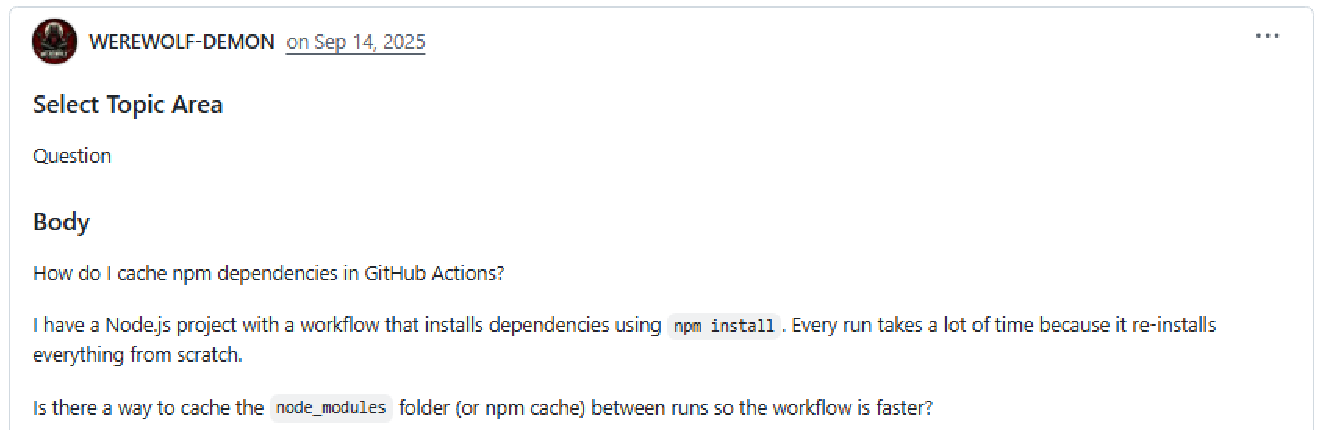
\includegraphics[width=\linewidth]{figures/ccs_S01_community_question_excerpt.pdf}
\par\smallskip
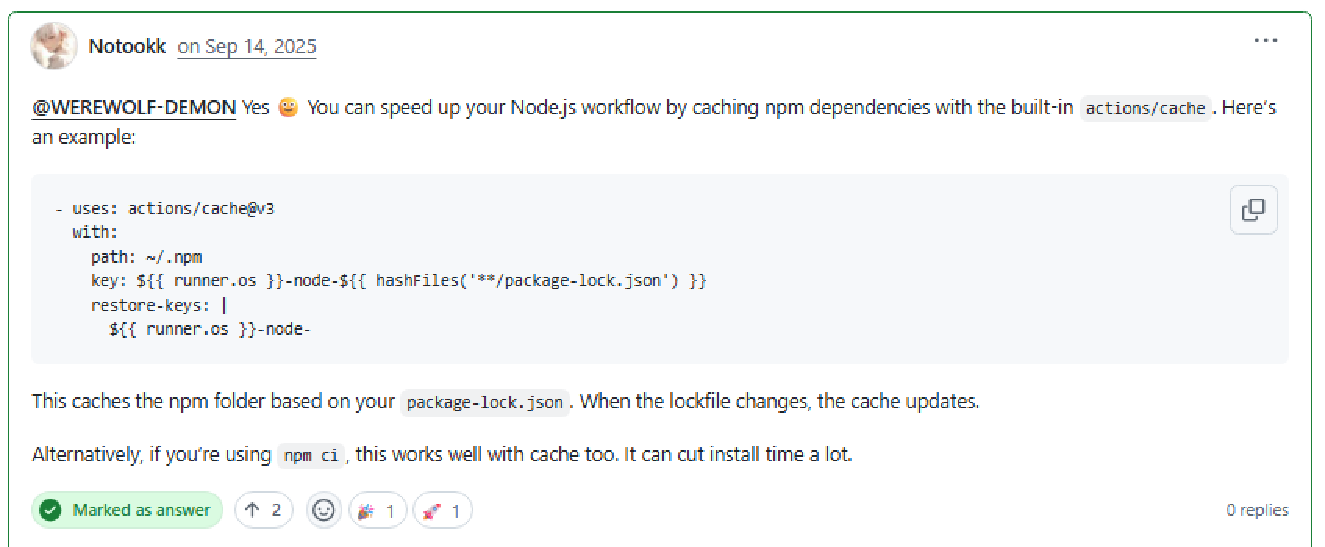
\includegraphics[width=\linewidth]{figures/ccs_S01_community_answer_excerpt.pdf}
\caption{Developer discussion of repeated npm dependency installation and caching recommendations (\href{https://github.com/orgs/community/discussions/173418}{\#173418}).}
\label{fig:ccs-dependency-report}
\end{figure}

\textbf{Detection rule.}
We identify jobs that install dependencies using npm, Yarn, pnpm, pip, Pipenv, Poetry, and uv (\texttt{uv sync} or \texttt{uv pip install}). A CCS is reported when a job performs one of these operations without a compatible explicit cache path or supported setup-action cache. For instance, caching provided by setup-node is recognized when \texttt{cache: npm} is configured, while setup-uv caching is recognized when \texttt{enable-cache} is set to \texttt{true} or \texttt{auto}. Jobs using custom setup actions that may implement caching internally are excluded from automatic reporting and recorded for review. Tool bootstrapping without dependency installation and unsupported package ecosystems are also excluded.



\FloatBarrier
\paragraph{\texttt{no\_docker\_layer\_cache}.}
Docker builds can reuse image layers when their inputs remain unchanged. Reusing those layers across workflow runs requires a cache that survives the build environment. This concern is covered by the GitLab CI/CD catalog and Docker's GitHub Actions caching guidance~\citep{urdih2026cache,docker_gha_cache_docs}. In Netflix/vmaf, the Docker job checks out the repository and directly executes \texttt{docker build} on a GitHub-hosted runner (Fig.~\ref{fig:ccs-docker-layer-code}). The job provides no visible layer-cache restoration or export mechanism. Local layer reuse within a build does not establish persistence between hosted workflow runs. Figure~\ref{fig:ccs-docker-layer-code}b illustrates a suggested configuration using Docker's GitHub Actions cache backend: \texttt{cache-from} imports cached layers, and \texttt{cache-to} exports them for subsequent builds~\citep{docker_gha_cache_docs}.

\begin{figure}[htbp]
\centering
\begin{lstlisting}[style=ccscase]
  1 name: Docker
  2 on:
  3   push:
  4   pull_request:
  5 
  6 jobs:
  7   docker:
|+|  8     runs-on: ubuntu-latest|/|
  9     steps:
 10       - uses: actions/checkout@v6
 11       - name: Build Docker Image
 12         run: |
|+| 13           docker build -t vmaf .|/|
\end{lstlisting}
\par\smallskip{\small (a)\par}
\begin{lstlisting}[style=ccscase,aboveskip=2pt,belowskip=3pt]
- uses: docker/setup-buildx-action@v3
- name: Build Docker Image
  uses: docker/build-push-action@v6
  with:
    context: .
    tags: vmaf
    load: true
|+|    cache-from: type=gha|/|
|+|    cache-to: type=gha,mode=max|/|
\end{lstlisting}
\par\smallskip{\small (b)\par}
\caption{\texttt{no\_docker\_layer\_cache} : \href{https://github.com/Netflix/vmaf/blob/30f472b146b9228f76c684360d6a976774290b5e/.github/workflows/docker.yml}{(a) Netflix/vmaf}; (b) suggested configuration.}
\label{fig:ccs-docker-layer-code}
\end{figure}


\textbf{Detection rule.}
We inspect Docker build commands and supported Buildx and Build Bake actions for reusable layer-cache configurations. We flag a job when it has no recognized caching mechanism, such as a local BuildKit cache directory, \texttt{cache-from}, \texttt{cache-to}, or a registry cache. Jobs with recognized warm-cache configurations are excluded. The rule checks for a visible caching configuration. Actual reuse depends on runtime conditions. It does not assess cache backend selection or migration.\footnote{For an example of runtime cache problems despite an existing layer-cache configuration, see GitHub Community discussion \#150429: \url{https://github.com/orgs/community/discussions/150429}.}



\FloatBarrier
\paragraph{\texttt{deprecated\_cache\_action}.}
The \texttt{deprecated\_cache\_action} smell occurs when a workflow uses a cache-action version that is no longer supported. Figure~\ref{fig:ccs-deprecated-code} illustrates this smell in MathiasGilson/Tailwind-Styled-Component, where line~14 references the deprecated \path{actions/cache@v2} release. GitHub's migration guidance warns that workflows using these deprecated releases will fail after the legacy cache service is retired and recommends upgrading to a supported release compatible with the new cache service~\citep{case_cache_migration_cutoff}.

\begin{figure}[htbp]
\centering
\begin{lstlisting}[style=ccscase]
  9 - uses: actions/checkout@v2
 10 - uses: actions/setup-node@v2
 11   with:
 12     node-version: '14'
 13 - name: Cache node modules
|+| 14   uses: actions/cache@v2|/|
 15   with:
 16     path: "**/node_modules"
 17     key: ${{ runner.os }}-modules-${{ hashFiles('**/yarn.lock') }}
 18     restore-keys: ${{ runner.os }}-modules-
 19 - name: Install Modules
 20   run: yarn install
\end{lstlisting}
\caption{\texttt{deprecated\_cache\_action} in \href{https://github.com/MathiasGilson/Tailwind-Styled-Component/blob/86be7109cc761123c142038efec7d54f2fc6b5f8/.github/workflows/test.yml}{MathiasGilson/Tailwind-Styled-Component}.}
\label{fig:ccs-deprecated-code}
\end{figure}


\textbf{Detection rule.}
We report explicit references to \path{actions/cache}, \path{actions/cache/restore}, and \path{actions/cache/save} that use a recognized v1 or v2 major release. The rule follows the version support status documented at the study cutoff. Third-party cache actions and references whose versions cannot be resolved statically are excluded.



\FloatBarrier
\paragraph{\texttt{no\_fallback\_cache}.}
\citet{urdih2026cache} identify missing fallback caches as a smell in GitLab CI/CD, noting that secondary keys allow jobs to reuse an alternative cache when the primary key is not found. In GitHub Actions, \texttt{restore-keys} serves a similar purpose by allowing broader matches when a dependency key changes but previously downloaded packages remain partially reusable~\citep{gha_cache_docs,gha_cache_strategies}. Omitting these keys or repeating the primary key provides no additional fallback matching. For example, the brocode/fw Cargo cache includes a lockfile hash in its primary key but omits \texttt{restore-keys} (Fig.~\ref{fig:ccs-fallback-code}a). The wasp-os/wasp-os pip cache instead supplies \texttt{restore-keys}, but repeats the entire hash-dependent primary key (Fig.~\ref{fig:ccs-fallback-code}b), leaving the matching scope unchanged.

\begin{figure}[htbp]
\centering
\begin{lstlisting}[style=ccscase,aboveskip=2pt,belowskip=3pt]
 16 - name: Cache folders
|+| 17   uses: actions/cache@v5|/|
 18   with:
 19     path: |
 20       ~/.cargo/registry
 21       ~/.cargo/git
 22       target
|+| 23     key: ${{ runner.os }}-cargo-${{ hashFiles('**/Cargo.lock') }}|/|
 24 
 25 - name: Check formatting, run clippy and test
 26   run: cargo fmt --all -- --check && cargo clippy -- -D warnings && cargo test
\end{lstlisting}
\par\smallskip{\small (a)\par}
\begin{lstlisting}[style=ccscase,aboveskip=2pt,belowskip=3pt]
 19 - name: Check the cached python downloads
 20   id:   cache-modules
 21   uses: actions/cache@v4
 22   env:
 23     cache-name: cache-toolchain
 24   with:
|+| 25     path: ~/.cache/pip|/|
|+| 26     key: ${{ runner.os }}-pip-${{ hashFiles('wasp/requirements.txt') }}|/|
|+| 27     restore-keys: ${{ runner.os }}-pip-${{ hashFiles('wasp/requirements.txt') }}|/|
    ... omitted ...
 35 - name: Install python modules
 36   id:   install-modules
 37   run: |
 38       pip3 install -r wasp/requirements.txt
\end{lstlisting}
\par\smallskip{\small (b)\par}
\caption{\texttt{no\_fallback\_cache}: \href{https://github.com/brocode/fw/blob/b01e51fa316d58d468d95e4bf0394d48bb35091e/.github/workflows/rust.yml}{(a) brocode/fw}; \href{https://github.com/wasp-os/wasp-os/blob/14cc0353b2eb9a3690fa23b265df04cb344a0e5c/.github/workflows/sim.yml}{(b) wasp-os/wasp-os}.}
\label{fig:ccs-fallback-code}
\end{figure}


\textbf{Detection rule.}
We examine eligible explicit dependency caches configured through \path{actions/cache} or \path{actions/cache/restore}. The \path{no_restore_key} subtype is reported when a primary \texttt{key} is present but \texttt{restore-keys} is absent or empty. The \path{ineffective_restore_key} subtype is reported when the fallback list contains the exact primary key without a broader effective prefix. A valid broader prefix satisfies the rule even if the list also contains an exact duplicate. Setup-action caches and cache content for which fallback reuse may be unsafe are excluded. Run-specific keys combined with broad fallback keys may also support intentional reuse of earlier entries~\citep{gha_cache_tips}. Both subtypes are counted as one CCS type.



\paragraph{\texttt{static\_cache\_key}.}
This smell arises when a cache key remains fixed as the inputs determining the cached content change. Because GitHub Actions cache entries are immutable, content added after a primary-key hit is not saved for subsequent runs~\citep{gha_cache_docs}. GitHub's caching guidance uses dependency-file hashes to make keys change with dependency updates, including hashes of \texttt{pom.xml} files for Maven~\citep{gha_cache_strategies,gha_cache_maven_example}. Crystal's CI guide likewise warns that static keys retain the initial cache contents despite later changes~\citep{crystal_ci_caching}. Figure~\ref{fig:ccs-static-key-code} illustrates this pattern in jetlinks/jetlinks-community, which caches \texttt{\string~/.m2} before a Maven build. The key, \texttt{jetlinks-community-maven-repository}, contains no component tied to the dependency declarations. When dependencies change, subsequent runs may therefore repeatedly download packages absent from the original entry without persisting them in the cache. A Gatsby developer reports the same limitation when attempting to update build caches stored under fixed keys.\footnote{The developer reports that the second build restores the caches but does not update them: \url{https://stackoverflow.com/questions/61078915}.} Fixed keys remain appropriate for content intended to stay unchanged, such as a tool whose version is explicitly encoded in the key.

\begin{figure}[htbp]
\centering
\begin{lstlisting}[style=ccscase,aboveskip=2pt,belowskip=3pt]
 21 - name: Cache Maven Repository
 22   uses: actions/cache@v4.2.3
 23   with:
|+| 24     path: ~/.m2|/|
|+| 25     key: jetlinks-community-maven-repository|/|
 26 - name: Build with Maven
 27   run: ./mvnw package -Dmaven.test.skip=true -Pbuild
\end{lstlisting}
\caption{\texttt{static\_cache\_key} in \href{https://github.com/jetlinks/jetlinks-community/blob/bb6e8a93ccbbb7fd91711a75c36d69472d5c2964/.github/workflows/pull_request.yml}{jetlinks/jetlinks-community}.}
\label{fig:ccs-static-key-code}
\end{figure}


\textbf{Detection rule.}
We inspect cache-writing configurations and resolve literal environment aliases where possible. We flag a key when it lacks an identifiable component that changes with the cached content. Read-only caches and fixed-version tool caches, such as those for LLVM, Clang, or CMake, are excluded when their keys contain recognizable version information. Manually updated keys for stable artifacts may also be intentional.



\paragraph{\texttt{overly\_specific\_cache\_key}.}
Keys can also change more often than the cached content requires. In argoproj/argo-rollouts, the explicit Go build-cache key contains \texttt{github.run\_id} and has no fallback (Fig.~\ref{fig:ccs-specific-key-code}). Each new workflow run therefore creates a distinct primary key for \texttt{\string~/.cache/go-build}, independently of changes to compilation inputs. The warning concerns this explicit key. The job also configures setup-go, which can provide caching independently. GitHub documents both key matching and deliberate strategies that combine unique write keys with broader restoration keys~\citep{gha_cache_action,gha_cache_tips}. The latter can preserve cross-run reuse and require a different interpretation.

\begin{figure}[htbp]
\centering
\begin{lstlisting}[style=ccscase,aboveskip=2pt,belowskip=3pt]
 48 - name: Restore go build cache
|+| 49   uses: actions/cache@v5|/|
 50   with:
|+| 51     path: ~/.cache/go-build|/|
|+| 52     key: ${{ runner.os }}-go-build-v1-${{ github.run_id }}|/|
 53 
 54 - name: Download all Go modules
 55   run: |
 56     go mod download
 57 - name: Test
 58   run: make test-unit
\end{lstlisting}
\caption{\texttt{overly\_specific\_cache\_key} in \href{https://github.com/argoproj/argo-rollouts/blob/16d28f8d6cdb35ec0e53b8ce8786c65f160bb1e2/.github/workflows/testing.yaml}{argoproj/argo-rollouts}.}
\label{fig:ccs-specific-key-code}
\end{figure}


\textbf{Detection rule.}
We report eligible cache-writing configurations whose keys contain run-specific values, such as \texttt{github.run\_id} or \texttt{github.run\_number}. The rule also covers workflow-definition information, including \path{github.workflow_ref}, \path{github.workflow_sha}, and hashes of files under \path{.github/workflows/}. Read-only caches and ordinary platform or tool-version dimensions are excluded. Commit identifiers, including \texttt{github.sha}, \texttt{github.event.after}, and pull-request head SHA, are not reported because they remain stable across reruns of the same commit. Workflow-related dimensions may also be necessary when changes to the workflow affect the cached content.



\flushbottom
\paragraph{\texttt{cache\_as\_artifact}.}
Caches support reuse across runs, while artifacts provide explicit transfer of workflow outputs~\citep{gha_cache_concepts,gha_artifact_docs}. In Alfresco/alfresco-content-app, the build job produces \texttt{dist/content-ce} and saves it under a key containing \texttt{github.run\_id}. A test job declaring \texttt{needs: [build]} restores the same key and path (Fig.~\ref{fig:ccs-transfer}). These relationships identify transfer of the current build's output through the cache. A separate community report describes storing build products in a cache that downstream jobs cannot retrieve. The accepted answer recommends artifacts (Fig.~\ref{fig:ccs-artifact-report}).\footnote{GitHub Community discussion \#26665, question by nyarly and accepted answer by airtower-luna: \url{https://github.com/orgs/community/discussions/26665}.} The concern is reliance on cache availability for a required producer--consumer handoff.

\textbf{Detection rule.}
We examine job dependencies declared through \texttt{needs} and identify caches containing artifact-like output paths or artifact-named keys. A CCS is reported when a downstream job restores a cache with the same key and overlapping paths as one written by an upstream job. Configurations using explicit artifact upload and download actions are excluded. The rule requires a visible transfer between dependent jobs and does not target outputs intended for reuse across workflow runs. Because the intended lifetime of cached content cannot always be established statically, reported cases indicate potential artifact-like cache usage.

\begin{figure}[!htbp]
\centering
\begin{lstlisting}[style=ccscase]
 37 build:
 38   name: 'build'
 39   runs-on: ubuntu-latest
 40   steps:
    ... omitted ...
 54     - run: npm run build -- $BUILD_OPTS
 55 
 56     - name: dist cache
 57       if: ${{ success() }}
|+| 58       uses: actions/cache/save@v5|/|
 59       with:
|+| 60         path: ./dist/content-ce|/|
|+| 61         key: cache-dist-${{ github.run_id }}|/|
 62 
 63 e2es-playwright:
|+| 64   needs: [build]|/|
    ... omitted ...
|+|126     - uses: actions/cache/restore@v5|/|
127       id: cache
128       with:
|+|129         path: ./dist/content-ce|/|
|+|130         key: cache-dist-${{ github.run_id }}|/|
\end{lstlisting}
\caption{\texttt{cache\_as\_artifact} in \href{https://github.com/Alfresco/alfresco-content-app/blob/85366003b55caa86719efe288c51ebb96665afa0/.github/workflows/run-e2e-with-env.yml}{Alfresco/alfresco-content-app}.}
\label{fig:ccs-transfer}
\end{figure}


\begin{figure}[!htbp]
\centering
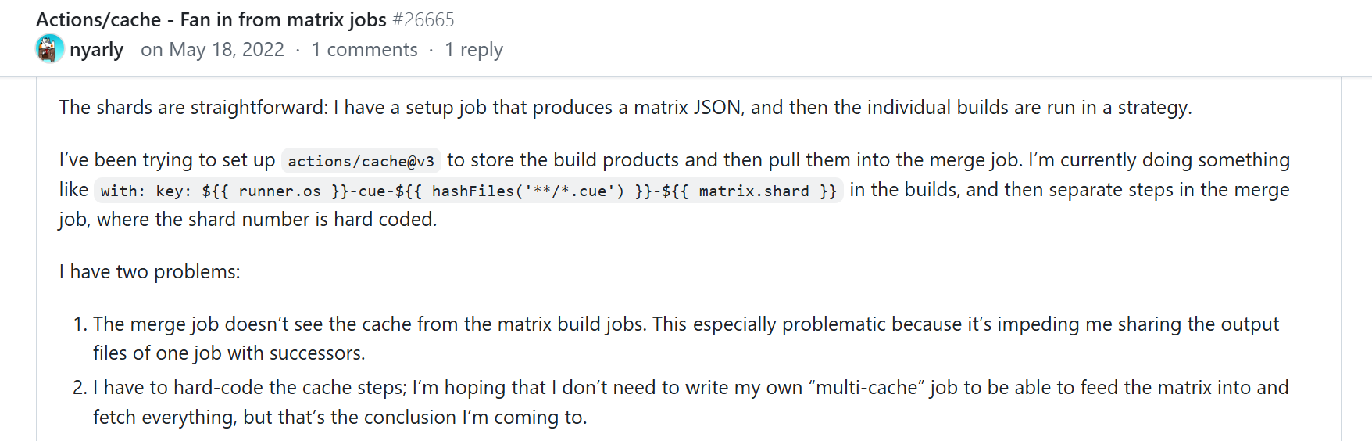
\includegraphics[width=\linewidth]{figures/ccs_S07_community_question_excerpt.pdf}
\par\smallskip
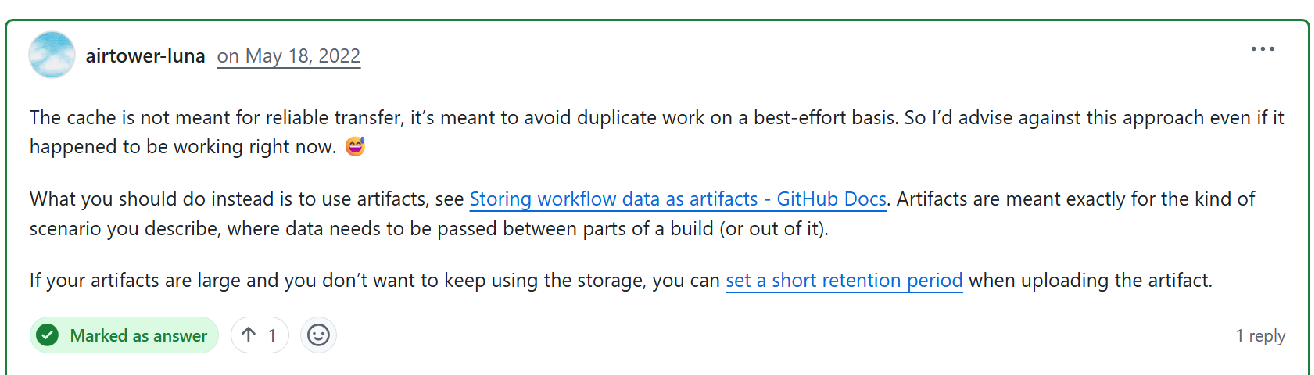
\includegraphics[width=\linewidth]{figures/ccs_S07_community_answer_excerpt.pdf}
\caption{Developer discussion of using caches to transfer build outputs between jobs (\href{https://github.com/orgs/community/discussions/26665}{\#26665}).}
\label{fig:ccs-artifact-report}
\end{figure}


\paragraph{\texttt{cache\_position\_error}.}
Cache restoration must precede the operation intended to reuse its contents. In extractus/article-extractor, \texttt{npm install}, linting, and tests all precede the explicit \texttt{actions/cache} step for \texttt{\string~/.npm} (Fig.~\ref{fig:ccs-position-error}). That restoration cannot serve the installation already completed at line~27. The example exposes an ordering relationship between a cache and its consumer, consistent with the documented restore/save lifecycle~\citep{gha_cache_action,gha_cache_docs}. It does not establish that the entire job lacks caching, because setup-action behavior can provide another mechanism.

\textbf{Detection rule.}
We classify cached resources and examine the order of checkout, cache-key prerequisites, restoration, cache producers, and consumers. Four subtypes are considered: \path{before_checkout}, when a cache key depends on repository content before checkout; \path{after_dependency_install}, when restoration follows the relevant dependency-installation operation; \path{after_cache_producer}, when restoration follows the operation producing the cached content; and \path{no_consumer}, when a runner-local build or intermediate cache has no observable consumer. The rule applies only when these relationships can be established statically. Tool and browser caches, such as Playwright and pre-commit caches, are excluded from generic ordering checks. Cache paths that do not depend on repository content may legitimately be restored before checkout.



\begin{figure}[!htbp]
\centering
\begin{lstlisting}[style=ccscase]
 24 
 25 - name: run npm scripts
 26   run: |
|+| 27     npm install|/|
 28     npm run lint
 29     #npm run build --if-present
 30     npm run test
 31 
|+| 32 - name: cache node modules|/|
|+| 33   uses: actions/cache@v5|/|
 34   with:
 35     path: ~/.npm
 36     key: ${{ runner.os }}-node-${{ hashFiles('**/package-lock.json') }}
 37     restore-keys: |
 38       ${{ runner.os }}-node-
\end{lstlisting}
\caption{\texttt{cache\_position\_error} in \href{https://github.com/extractus/article-extractor/blob/c94926a53c87e15730a72bd56d04daba2e1fd47d/.github/workflows/ci-test.yml}{extractus/article-extractor}.}
\label{fig:ccs-position-error}
\end{figure}


\paragraph{\texttt{unreachable\_cache\_write}.}
An explicit save step can be present but unreachable under the workflow's trigger and conditions. In mozilla-mobile/mozilla-vpn-client, the linter workflow accepts only \texttt{pull\_request} events, while its conda-cache save step requires \texttt{github.event\_name == 'push'} (Fig.~\ref{fig:ccs-unreachable-write}). The event predicate is false for every permitted invocation, regardless of the preceding restore result. Because split cache actions persist new content through an explicit save operation~\citep{gha_cache_action,gha_cache_strategies}, this contradiction prevents that step from populating the cache. The example provides a statically decidable condition conflict without inferring values of runtime outputs.

\textbf{Detection rule.}
We inspect explicit \path{actions/cache/save} steps for contradictions visible in workflow YAML. These include statically false job or step conditions, event conditions inconsistent with the workflow triggers, and mutually exclusive job and step conditions. The rule also identifies references to cache-output steps that are undefined within the job. Conditions depending on runtime outputs are not evaluated. Undefined references are treated as potential configuration problems rather than conclusive evidence that a save step cannot execute.

\begin{figure}[!htbp]
\centering
\begin{lstlisting}[style=ccscase]
  1 name: Linters (clang, l10n, colors)
  2 on:
  3   # Triggers the workflow on pull request events but only for the main branch
|+|  4   pull_request:|/|
  5     branches:
  6       - main
  7       - "releases/**"
  8     types:
  9       - opened
 10       - synchronize
 11       - reopened
    ... omitted ...
 84   ktlint:
 85     name: Run ktLint
 86     runs-on: ubuntu-latest
    ... omitted ...
 98       - name: Cache conda packages
 99         id: conda-cache
100         uses: actions/cache/restore@27d5ce7f107fe9357f9df03efb73ab90386fccae # v5.0.5
    ... omitted ...
115       - name: Save conda package cache
|+|116         uses: actions/cache/save@27d5ce7f107fe9357f9df03efb73ab90386fccae # v5.0.5|/|
|+|117         if: ${{ github.event_name == 'push' && steps.conda-cache.outputs.cache-hit != 'true' }}|/|
118         with:
119           path: ~/conda_pkgs_dir
120           key: android-conda-packages-${{ hashFiles('env-android.yml', 'requirements.txt') }}
\end{lstlisting}
\caption{\texttt{unreachable\_cache\_write} in \href{https://github.com/mozilla-mobile/mozilla-vpn-client/blob/75a233a98bc1cf023644f127745489d26a3c4b5d/.github/workflows/linters.yaml}{mozilla-mobile/mozilla-vpn-client}.}
\label{fig:ccs-unreachable-write}
\end{figure}



\FloatBarrier
\paragraph{\texttt{redundant\_cache\_update}.}
\citet{urdih2026cache} identify redundant cache updates when multiple jobs update shared cached files although a single writer would suffice. For example, the Java 17, 21, and 25 matrix instances in http-kit/http-kit cache \texttt{\string~/.m2/repository} using the same \texttt{project.clj}-based key (Fig.~\ref{fig:ccs-redundant-update}). Each instance runs \texttt{lein test-ci} and retains the cache action's automatic save behavior. If the instances miss the primary key, they may compete to populate the same cache entry after successful completion. GitHub Actions skips saving on a primary-key hit and does not overwrite existing entries~\citep{gha_cache_action,gha_cache_docs}. GitHub's caching guidance documents a corresponding strategy in which a centralized job saves the cache and other jobs use restore-only actions~\citep{gha_cache_strategies}.

\textbf{Detection rule.}
We resolve statically identifiable environment and matrix values and examine job dependencies to identify cache writers that may execute concurrently. A CCS is reported when these writers use equivalent expanded keys. Restore-only operations are not treated as writers. The rule also excludes configurations using \texttt{lookup-only} or \texttt{fail-on-cache-miss} to limit automatic reporting. These exclusions define the rule's scope. The \texttt{lookup-only} option does not itself disable saving~\citep{gha_cache_action}. The rule accounts for \texttt{needs} dependencies, statically resolvable mutually exclusive job conditions, and matrix configurations. Sequential jobs and jobs that only restore caches are excluded. Reported cases indicate possible redundant cache population rather than confirmed concurrent writes.

\begin{figure}[!htbp]
\centering
\begin{lstlisting}[style=ccscase]
  4 jobs:
  5   tests:
  6     strategy:
  7       matrix:
|+|  8         java: ['17', '21', '25']|/|
|+|  9         os: [ubuntu-latest]|/|
 10 
 11     runs-on: ${{ matrix.os }}
    ... omitted ...
 23       - uses: actions/cache@v5
|+| 24         id: cache-deps|/|
 25         with:
|+| 26           path: ~/.m2/repository|/|
|+| 27           key: deps-${{ hashFiles('project.clj') }}|/|
 28           restore-keys: deps-
 29 
|+| 30       - run: lein test-ci|/|
\end{lstlisting}
\caption{\texttt{redundant\_cache\_update} in \href{https://github.com/http-kit/http-kit/blob/7bd0a06ae2d5e50a44ec38fb0f672897352cfe8d/.github/workflows/main-tests.yml}{http-kit/http-kit}.}
\label{fig:ccs-redundant-update}
\end{figure}



\paragraph{\texttt{overlapping\_cache\_mechanisms}.}
A job can assign the same cached resource to multiple mechanisms. OpenAPITools/openapi-style-validator enables setup-java's Gradle cache and separately configures \texttt{actions/cache} for \texttt{\string~/.gradle/caches} (Fig.~\ref{fig:ccs-overlapping-mechanisms}). The setup-java implementation at the referenced version caches both that directory and \texttt{\string~/.gradle/wrapper}.\footnote{The setup-java v4.2.2 implementation lists the Gradle cache paths in \path{src/cache.ts}, lines 31--35: \url{https://github.com/actions/setup-java/blob/v4.2.2/src/cache.ts\#L31-L35}.} The intersection therefore establishes overlapping cache management within one job. This concern extends documented setup-action and explicit caching support~\citep{gha_cache_docs}, alongside prior observations of cache-configuration maintenance~\citep{hasan2026caching}. Distinct resources cached by different mechanisms do not exhibit this overlap.

\begin{figure}[!htbp]
\centering
\begin{lstlisting}[style=ccscase]
 14 - name: Set up JDK
 15   uses: actions/setup-java@v4.2.2
 16   with:
 17     distribution: 'adopt'
 18     java-version: 11
|+| 19     cache: 'gradle'|/|
 20 - name: print Java version
 21   run: java -version
 22 - name: Cache Gradle packages
|+| 23   uses: actions/cache@v4.3.0|/|
 24   with:
|+| 25     path: ~/.gradle/caches|/|
 26     key: ${{ runner.os }}-gradle-${{ hashFiles('**/*.gradle') }}
 27     restore-keys: ${{ runner.os }}-gradle
 28 - name: Build
 29   run: ./gradlew build --info --stacktrace
\end{lstlisting}
\caption{\texttt{overlapping\_cache\_mechanisms} in \href{https://github.com/OpenAPITools/openapi-style-validator/blob/13eb4eb01c11b7de4840867f06f79f97d9e14e07/.github/workflows/build.yml}{OpenAPITools/openapi-style-validator}.}
\label{fig:ccs-overlapping-mechanisms}
\end{figure}


\textbf{Detection rule.}
We identify supported setup actions with built-in caching enabled and compare their inferred package-manager cache paths with those of explicit \path{actions/cache} steps. We flag a job when both mechanisms target the same supported cache content. Configurations that cache distinct resources are excluded, even when they use the same package manager. The rule identifies overlapping cache management without assuming that the overlap causes data corruption.



\subsubsection{Detector Implementation}
\label{subsec:detector}

We implement the 11 detection rules as a Python static analyzer of workflow configurations. The detector parses workflow YAML files into jobs and ordered steps, identifying explicit cache operations and supported setup-action caching configurations. For each cache operation, it records the paths, key, operation type, and step position. It also identifies package-manager operations, checkout steps, and dependencies between jobs.

To apply the rules, the detector resolves supported environment-variable references and expands static matrices where needed, including \texttt{include} and \texttt{exclude} entries. It uses the extracted information to identify cache consumers and producers, check step ordering, and compare cache configurations across jobs. Each finding reports the CCS type, affected jobs, and supporting configuration evidence.

The detector analyzes configuration and command text without executing shell commands or recursively inspecting reusable workflows and custom actions. Each rule specifies how behavior that cannot be resolved affects reporting. For \path{no_dependency_cache}, the detector omits findings for jobs with recognized custom setup actions that may encapsulate caching. It also omits findings for a package manager when a supported setup action's caching state remains unknown. These cases remain unresolved and do not establish that caching is enabled.

\subsection{Constructing the Study Datasets}
\label{sec:data-construction}

We construct a workflow snapshot dataset for RQ1 and a linked run dataset for RQ2.1 and RQ2.2. RQ2.3 uses separate historical archives to compare resource use across configuration changes within the same workflow.

\datastepheading{Repository selection and data collection}

We use the GHALogs repository list~\citep{ghalogs2024,ghalogs_msr25} to identify candidate repositories. We collect repository metadata for these candidates through the GitHub API. We exclude forks and archived repositories and require more than 100 stars, more than 100 commits, and more than 50 workflow runs recorded over a 90-day period. These criteria focus the study on established projects with recent CI activity, consistent with prior work that screens projects by popularity and CI usage~\citep{urdih2026cache}.

We independently collect workflow YAML files under \texttt{.github/workflows/} and workflow-run records through the GitHub REST API. We also retrieve information on changes to these workflow files. We use 9 June 2026 at 23:59:59 UTC as the study cutoff and retrieve the latest default-branch workflow files available at or before this time. The collection yields 131,009 source workflow records.

\datastepheading{Workflow dataset construction}

RQ1 examines the latest workflow configurations available at the study cutoff. We identify repositories by their GitHub IDs and workflows by repository ID and normalized file path. Merging 11,807 duplicate workflow records and removing 319 records whose repositories could not be identified yields 118,883 distinct workflows.

We exclude 481 workflows with missing or unusable detection results, leaving 118,402 workflows from 19,324 repositories for RQ1. We measure CCS prevalence and co-occurrence at the workflow level and aggregate findings by repository for repository-level analyses.

\datastepheading{Linking workflow configurations to runs}

For RQ2.1 and RQ2.2, we link the workflow configurations described above to their run records. We retain completed runs on each repository's default branch, created during the 30 days ending at the study cutoff. These runs must be triggered by \texttt{push}, \texttt{schedule}, or \texttt{workflow\_dispatch}. We remove duplicate records using repository ID, run ID, and attempt number.

We link run records to workflow files using GitHub workflow IDs. If a collected workflow record has no ID, we look for run records from the same repository that refer to the same workflow file. We retain the workflow only when these records identify a single workflow ID.

We associate each workflow's latest configuration with runs created after its last modification. Specifically, runs must be created on or after both the workflow file's last modification and the start of the analysis window, and no later than the cutoff. Commits that do not modify the workflow file do not affect this association. We use workflow IDs and file modification times for matching, without retrieving workflow YAML at each run's \texttt{head\_sha}.

\begin{table}[htbp]
\centering\small
\caption{Outcome-specific RQ2 samples}
\label{tab:rq2-screening-flow}
\begin{tabular}{lrrr}
\hline
\textbf{Sample} & \textbf{Versions} & \textbf{Repositories} & \textbf{Runs} \\
\hline
All linked runs & 51,179 & 14,710 & 1,093,639 \\
Usable detection results & 51,097 & 14,695 & 1,091,978 \\
Completed-run duration & 50,985 & 14,690 & 1,089,617 \\
Workflow-run success & 50,460 & 14,632 & 1,047,015 \\
\hline
\end{tabular}
\end{table}

We exclude runs whose workflow configurations lack usable detection results. We then select the duration and success samples separately, as summarized in Table~\ref{tab:rq2-screening-flow}.

\datastepheading{Historical comparison sample construction}

RQ2.3 uses archived workflow configurations, run records, and job-level execution data to compare resource use across configuration changes within the same workflow. We include a comparison when a CCS type changes detection status and successful default-branch runs with complete resource data are available on both sides of the change. We retain all qualifying archived runs without imposing a fixed 30-day window. The final sample contains 166 configuration-change events from 88 repositories and 1,268 successful run attempts with complete resource data. The retained runs were created between 22 August 2025 and 9 June 2026. Section~\ref{sec:analysis-methods} details the matching procedure and resource-data requirements.

\subsection{Evaluating the Detector}
\label{sec:validation-design}

We randomly sample 383 workflows from the 118,402 workflows in the study dataset for manual evaluation. We determine the sample size using Cochran's formula with a finite population correction~\citep{cochran1977sampling}, a 95\% confidence level, a 5\% margin of error, and an assumed proportion of 0.5. Two annotators independently inspect each workflow against the CCS definitions in Section~\ref{sec:taxonomy} and label the presence or absence of the 11 CCS types. They discuss disagreements to establish the final reference annotations.

We compare the detector's predictions with the reference annotations at the workflow level and report precision, recall, and F1 for each CCS type. With TP, FP, and FN denoting workflow-level true positives, false positives, and false negatives, respectively, we compute these metrics as follows:
\[
\mathrm{Precision}=\frac{\mathrm{TP}}{\mathrm{TP}+\mathrm{FP}},\qquad
\mathrm{Recall}=\frac{\mathrm{TP}}{\mathrm{TP}+\mathrm{FN}},\qquad
\mathrm{F1}=\frac{2\,\mathrm{Precision}\,\mathrm{Recall}}
{\mathrm{Precision}+\mathrm{Recall}}.
\]

\subsection{Analyzing Prevalence and Workflow Outcomes}
\label{sec:analysis-methods}

\paragraph{Measuring prevalence and comparing contexts (RQ1.1).}

We report CCS frequency at the instance, workflow, and repository levels. An instance is a detector finding. A workflow is counted once per CCS type, regardless of the number of findings. A repository is counted once per type when at least one of its workflows contains that CCS. Overall prevalence uses the common denominators of 118,402 workflows and 19,324 repositories. Supplementary rates use observable configuration metadata to define rule-specific opportunity denominators.

We describe CCS distributions by workflow triggers and roles, repository primary language and features, and the fraction of affected workflows within each repository. Because \path{no_dependency_cache} (NDC) covers observable npm-compatible and Python-compatible installations, we also report the union of the other 10 CCS types. This comparison retains all workflows in the denominator and the same repository-primary-language groups. Separately, we describe NDC among workflows with supported installation operations, grouped as npm-compatible, Python-compatible, or mixed. These groups describe dependency operations, which may differ from the repository's primary language.

For repository-feature comparisons, the reference group contains 8,796 repositories with no detected CCS in any analyzed workflow. Each CCS-specific group contains repositories with at least one workflow exhibiting that type. Repositories can belong to several groups because CCS types can co-occur. We compare stars, contributors, workflow counts, recorded 90-day workflow runs, and commits on the $\log_{10}(x+1)$ scale to accommodate their skewed distributions. Each split violin uses the same reference group. Groups describe repository context and are defined by observed CCS presence, rather than rule-specific eligibility.

Following CI studies that combine nonparametric comparisons with effect sizes~\citep{ghaleb2019empirical}, we use two-sided Mann--Whitney $U$ tests for repository-feature distributions. Each repository contributes one observation per feature in a comparison. The target and reference groups are disjoint. We use the asymptotic, tie-corrected test with continuity correction and apply Holm correction across all 55 comparisons (11 CCS types $\times$ five features). This correction accommodates dependence arising from the shared reference and overlapping target groups. We report Cliff's $\delta=2U/(n_\mathrm{target}n_\mathrm{reference})-1$, with $U$ oriented toward the target group. Positive values indicate larger target-group values. The effect size $\delta$ measures distributional dominance rather than a difference in medians. Tests use raw values, whose ranks are preserved by the plotted logarithmic transformation. Missing feature values are omitted only from the corresponding comparison. These post-hoc context comparisons are exploratory. The replication output records sample sizes, medians, $U$, raw and corrected $p$-values, and $\delta$ for all 55 comparisons.

We classify workflow roles using job identifiers and explicit job names, following prior work~\citep{bouzenia2024resource}. We lowercase these strings, remove parenthesized platform or matrix details, and match simplified task tokens as substrings. Workflows with multiple recognized categories are labeled ``mixed''. Those with no recognized category are labeled ``other''. Classification uses job names alone.

\paragraph{Measuring multiplicity and co-occurrence (RQ1.2).}

Following prior work on configuration-smell distributions~\citep{wu2020dockerfilesmells}, we count the distinct CCS types in each workflow and examine their pairwise co-occurrence. For each pair, we report the number and share of workflows containing both types. We also compute the Jaccard index, dividing the number containing both by the number containing either type.

\subsubsection{Estimating Associations and Summarizing Resource Use}
\label{sec:rq2-common}

\paragraph{Common outcome samples.} We fit one model per outcome using all workflow versions with usable detector states and qualifying runs. Each model includes the 11 CCS indicators jointly. Invariant indicators are omitted because their coefficients cannot be estimated. We do not restrict the regression sample to each rule's detection preconditions. Each coefficient therefore compares versions with and without a reported CCS in the full outcome sample, conditional on the remaining indicators and controls. Absence of a report does not establish that a configuration is applicable or free of caching concerns. Duration is the primary outcome, and workflow-run success is secondary.

CCS labels are assigned to workflow versions, while outcomes are measured for individual runs. Within each outcome sample, we weight each run by the inverse of its version's run count. Each version thus contributes a total weight of one to the corresponding model. This retains repeated runs while balancing versions with different execution frequencies. We cluster standard errors by repository to account for dependence among its runs.

\paragraph{Selecting control variables.}
Following empirical CI studies that explain configuration and execution factors before interpreting model coefficients~\citep{ghaleb2019empirical,ghaleb2022studying}, we control for workload, execution environment, and timing. Both outcome models use the control vector $\mathbf{X}_{iv}$, where $i$ indexes runs and $v$ indexes workflow versions. Table~\ref{tab:regression-controls} explains why each group is included. Controls are derived from workflow configurations and run metadata rather than outcome-dependent classifications. Including all CCS indicators jointly accounts for their measured co-occurrence.

\begin{table}[htbp]
\centering\small
\caption{Control variables and their rationale}
\label{tab:regression-controls}
\begin{tabularx}{\linewidth}{@{}p{0.37\linewidth}Y@{}}
\hline
\textbf{Controls} & \textbf{Reason for inclusion} \\
\hline
Job count; non-cache step count; matrix presence & Represent workflow size and configured parallel workload. Explicit cache-action steps are excluded from the step count to avoid making this measure depend directly on cache configuration. \\
Workflow role; dependency ecosystem & Distinguish task and toolchain requirements, which can differ in baseline duration and failure frequency. \\
Runner operating system; hosting type & Account for differences in platform, execution environment, and runner provisioning. \\
Run event; observation week & Distinguish triggered workloads and shared temporal variation within the 30-day window. \\
\hline
\end{tabularx}
\end{table}

We transform job and non-cache step counts as $\log(1+x)$ and standardize them over the distinct version--event--week design rows within each outcome sample. Workflow role is inferred from workflow and job names and the workflow path. Ecosystem is inferred from setup actions and commands. Mixed and unknown categories are retained. Categorical variables use indicator coding, with the most frequent design-row level as the reference. Binary coefficients compare presence with absence, conditional on the other included variables. Invariant predictors are omitted. Both models use unpenalized weighted least squares. Repository clustering adjusts uncertainty for dependence among runs. It does not remove unmeasured repository differences.

\paragraph{Statistical inference.} We use repository-clustered sandwich standard errors with a $G/(G-1)$ correction, where $G$ is the number of repositories in the outcome sample~\citep{cameron2015clusterrobust}. Duration coefficients use two-sided normal-reference Wald tests. The success model uses two-sided $t$ tests with $G-1$ degrees of freedom. Duration intervals are exponentiated to the ratio scale. Success intervals remain on the probability-difference scale. We apply Benjamini--Hochberg false-discovery-rate correction separately to the 10 estimable CCS coefficients in each primary outcome model~\citep{benjamini1995fdr}. Unreachable cache writes have no exposed version and contribute no test. An association is statistically significant when $q<0.05$. The reported 95\% intervals are pointwise. Control-variable tests are outside the CCS-level correction families.

\paragraph{Assessing model fit.}
We assess predictor redundancy using design-matrix rank, variance-inflation factors (VIFs), and the condition number of the weighted, standardized predictor matrix. Invariant or linearly dependent columns are omitted, and any affected CCS coefficient is marked as not estimable.

For duration, version-weighted $R^2$ measures the fraction of variation in log seconds explained relative to a weighted-mean prediction. RMSE summarizes residual error in log seconds. For success, we report weighted $R^2$, mean squared error, and the proportion of fitted values outside $[0,1]$, without clipping predictions. These measures summarize in-sample fit rather than predictive performance. Online Resource~2 reports diagnostics, full coefficients, and repository-clustered uncertainty.

As a sensitivity analysis, we fit the same log-duration model to successful runs only. Inference uses the sandwich estimates described above, without bootstrap resampling. Estimates for CCS present in fewer than 30 versions or 10 repositories are treated as exploratory, and exposure counts are reported to identify sparse comparisons. The models estimate adjusted associations in observational data.

\paragraph{Modeling completed-run duration (RQ2.1).}

We fit a weighted linear model to the log duration of completed runs with valid positive durations:
\[
\log(D_{iv}) = \alpha_0 + \sum_{j=1}^{11}\alpha_j S_{jv} + \boldsymbol{\delta}^{\mathsf{T}}\mathbf{X}_{iv} + \epsilon_{iv}.
\]
Here, $D_{iv}$ is the duration in seconds of run $i$ from version $v$, and $S_{jv}$ indicates CCS type $j$. The sample includes completed runs with valid durations greater than zero and no more than 35 days. We report $\exp(\alpha_j)$ as the adjusted duration ratio. Values above one indicate longer duration, and $100\{\exp(\alpha_j)-1\}$ gives the percentage difference on the modeled multiplicative scale. The ratio compares conditional geometric means. For example, a ratio of 1.20 corresponds to 20\% longer modeled duration at the same included covariate values.

\paragraph{Modeling workflow-run success (RQ2.2).}

We fit a weighted linear probability model (LPM), an approach also used to analyze binary code-review outcomes~\citep{murphyhill2023systemic}:
\[
Y_{iv} = \beta_0 + \sum_{j=1}^{11}\beta_j S_{jv} + \boldsymbol{\gamma}^{\mathsf{T}}\mathbf{X}_{iv} + u_{iv}.
\]
The indicator $Y_{iv}$ equals one for a \texttt{success} conclusion and zero for \texttt{failure}, \texttt{startup\_failure}, or \texttt{timed\_out}. Other conclusions are excluded. We report $100\beta_j$ as the adjusted success-probability difference in percentage points. For example, $\beta_j=-0.04$ corresponds to a four-percentage-point lower modeled success probability. Unlike ordinary logistic estimation, weighted least squares can yield a finite coefficient when all exposed runs fail, provided the design is identifiable. Its linear specification may produce fitted values outside $[0,1]$, which we report as a model limitation.

\paragraph{Measuring runner time and estimating cost (RQ2.3).}

RQ2.3 compares resource use across historical versions of the same workflow when a CCS type changes detection status. We reuse locally archived workflow histories, run records, and exact-attempt job data, rather than the latest-version regression cohort. The detector identifies 1,934 candidate changes involving the 11 studied types. A comparison requires a change from detected to undetected, or vice versa, within the same repository and workflow identity. We do not require other tasks, jobs, runner settings, or CCS types to remain unchanged. The undetected side need not satisfy the rule's detection preconditions and therefore does not necessarily represent a verified repair.

We assign default-branch runs to each version's validity interval and retain completed, successful runs with complete resource records on both sides. Available execution-content evidence is used to exclude confirmed version mismatches. Exact content confirmation is not required when only interval evidence is available. All qualifying archived runs are retained, without a fixed number per side or a 30- or 90-day comparison window. Because the archives include targeted collections, this sample does not represent a random or complete set of historical changes.

Runner-allocated VM time is the sum of \texttt{completed\_at} minus \texttt{started\_at} across jobs with a positive numeric \texttt{runner\_id}. Jobs without an allocated runner contribute zero. We exclude runs with unavailable exact-attempt jobs, invalid allocated-job timestamps, self-hosted runners, or unknown pricing categories. We estimate cost using the fixed reference-pricing convention of \citet{bouzenia2024resource}:
\[
C_r=\sum_{j\in r}\left\lceil \frac{t_j}{60}f_{o(j)}\right\rceil \times 0.008,
\]
where $t_j$ is allocated job time in seconds, and $f_{o(j)}$ equals 1 for Linux, 2 for Windows, and 10 for macOS. Rounding is applied separately to each job. This historical reference measure excludes storage and does not represent actual charges or current runner prices.

For each change event, we subtract the undetected side's mean per-run resource use from the detected side's mean. For each CCS type, we average event differences within repositories and then give repositories equal weight. We report pointwise 95\% percentile intervals from 2,000 repository bootstrap samples, using seed 20261019. We do not report a population interval for a single repository or treat intervals as multiplicity-adjusted tests.

To express these differences at a monthly scale, we use audited, complete run archives for April and May 2026. Within each workflow, we average historical event differences and multiply by that workflow's actual successful default-branch run count in each month. We sum the compared workflows within each repository, average the two months, and then average repositories with equal weight. Workflows without complete frequency coverage are omitted from this calculation, rather than assigned zero runs. The result is a monthly equivalent at observed frequencies, assuming historical per-run differences transfer to those months. It is not observed monthly expenditure attributable to CCS.

\section{Results}
\label{sec:results}

We first report detector evaluation, followed by CCS occurrence patterns (RQ1) and associations with workflow outcomes and resource use (RQ2). Unless stated otherwise, prevalence estimates use the canonical workflow frame, whereas the outcome analyses use the version-aligned run cohort.

\subsection{Detector Validation Results}
\label{subsec:detector-validation}

Table~\ref{tab:detector-validation} reports workflow-level precision, recall, and F1 for the 11 CCS types on the 383 manually annotated workflows described in Section~\ref{sec:validation-design}.

\begin{table}[htbp]
\centering
\caption{Workflow-level evaluation of the 11 detector rules against manual annotations of 383 workflows}
\label{tab:detector-validation}
\scriptsize
\begin{tabular}{lrrrrrr}
\hline\noalign{\smallskip}
\textbf{CCS} & \textbf{TP} & \textbf{FP} & \textbf{FN} & \textbf{Precision} & \textbf{Recall} & \textbf{F1} \\
\noalign{\smallskip}\hline\noalign{\smallskip}
Missing dependency cache & 51 & 2 & 5 & 96.23\% & 91.07\% & 93.58\% \\
Missing fallback matching & 171 & 10 & 0 & 94.48\% & 100.00\% & 97.16\% \\
Redundant cache update & 54 & 0 & 3 & 100.00\% & 94.74\% & 97.30\% \\
Cache placement error & 16 & 1 & 2 & 94.12\% & 88.89\% & 91.43\% \\
Missing Docker layer cache & 42 & 2 & 9 & 95.45\% & 82.35\% & 88.42\% \\
Deprecated cache action & 36 & 0 & 0 & 100.00\% & 100.00\% & 100.00\% \\
Cache used as an artifact & 40 & 1 & 3 & 97.56\% & 93.02\% & 95.24\% \\
Overlapping mechanisms & 27 & 0 & 3 & 100.00\% & 90.00\% & 94.74\% \\
Static cache key & 57 & 1 & 2 & 98.28\% & 96.61\% & 97.44\% \\
Overly specific cache key & 43 & 0 & 1 & 100.00\% & 97.73\% & 98.85\% \\
Unreachable cache write & 4 & 0 & 0 & 100.00\% & 100.00\% & 100.00\% \\
\noalign{\smallskip}\hline
\end{tabular}
\par\smallskip
\parbox{\linewidth}{\footnotesize\emph{Note.} Missing dependency caching is evaluated on 341 workflows within the rule's scope. The other rules are evaluated on all 383 workflows.}
\end{table}

Precision ranged from 94.12\% to 100.00\%, and recall ranged from 82.35\% to 100.00\%. Missing Docker layer caching had nine false negatives, the most among the 11 rules. Unreachable cache writes had only four positive reference workflows, limiting the evidence behind its perfect scores.

\subsection{Prevalence and Occurrence Patterns (RQ1)}

\subsubsection{Prevalence across Workflows and Repositories (RQ1.1)}

At least one CCS was detected in 26,388 of 118,402 workflows (22.29\%), covering 10,528 of 19,324 repositories (54.48\%). Missing dependency caching was the most prevalent type, followed by missing fallback matching and missing Docker layer caching (Table~\ref{tab:smell-prevalence}).

\begin{table}[htbp]
\centering\small
\caption{CCS prevalence across workflows and repositories}
\label{tab:smell-prevalence}
\begin{tabularx}{\linewidth}{@{}Yrr@{}}
\hline
\textbf{CCS} & \textbf{Workflows (\%)} & \textbf{Repositories (\%)} \\
\hline
Missing dependency cache & 16,138 (13.63) & 6,976 (36.10) \\
Missing Docker layer cache & 3,852 (3.25) & 2,343 (12.12) \\
Deprecated cache action & 463 (0.39) & 249 (1.29) \\
Missing fallback matching & 5,757 (4.86) & 3,007 (15.56) \\
Static cache key & 1,720 (1.45) & 1,142 (5.91) \\
Overly specific cache key & 661 (0.56) & 405 (2.10) \\
Cache used as an artifact & 147 (0.12) & 116 (0.60) \\
Cache placement error & 872 (0.74) & 528 (2.73) \\
Unreachable cache write & 4 ($<0.01$) & 4 (0.02) \\
Redundant cache update & 1,970 (1.66) & 1,460 (7.56) \\
Overlapping mechanisms & 660 (0.56) & 407 (2.11) \\
\hline
Any CCS & 26,388 (22.29) & 10,528 (54.48) \\
\hline
\end{tabularx}
\par\smallskip\parbox{\linewidth}{\footnotesize\emph{Note.} Cells report counts with percentages. Denominators are 118,402 workflows and 19,324 repositories. Types can co-occur, so their counts do not sum to the union. Per-instance counts are retained in the replication data.}
\end{table}

Overall prevalence uses 118,402 workflows and 19,324 repositories as denominators. Instance counts include every detector finding, whereas workflow counts include each affected workflow once per CCS type. Repository counts include each affected repository once. Supplementary rates instead use the workflows or repositories eligible for each rule.



\paragraph{Repository language.}
We group workflows by repository primary language, retaining all eight language groups, including ``Other.'' Table~\ref{tab:ecosystem-distribution} reports the prevalence of any CCS, the union excluding missing dependency caching (S1), and S1 separately. The complete 11-rule cross-tabulation and non-NDC sensitivity counts are available in \texttt{rq1\_ecosystem\_distribution.csv} and \texttt{rq1\_ecosystem\_non\_ndc\_sensitivity.csv}, respectively.

\begin{table}[htbp]\caption{CCS prevalence by repository primary language, with and without NDC}\label{tab:ecosystem-distribution}\centering\small
\begin{tabular}{lrrrr}\hline
Primary language & Workflows & Any CCS & Without S1 & S1\\\hline
PHP & 4,503 & 16.32\% & 11.48\% & 5.49\% \\
Rust & 8,140 & 16.55\% & 10.72\% & 6.93\% \\
Java/Kotlin & 11,319 & 15.87\% & 11.40\% & 5.12\% \\
Other & 14,641 & 15.42\% & 8.26\% & 7.75\% \\
Go & 15,679 & 15.70\% & 12.42\% & 3.84\% \\
C/C++ & 16,614 & 21.06\% & 10.64\% & 12.12\% \\
Python & 21,236 & 37.81\% & 9.00\% & 31.26\% \\
JavaScript/TypeScript & 26,270 & 23.84\% & 8.31\% & 16.59\% \\\hline
\end{tabular}\par\smallskip\noindent\parbox{\linewidth}{\footnotesize\emph{Note.} Percentages use the workflow count in each row as their denominator. ``Without S1'' is the union of the other 10 rules, not the sum of their rates. S1 = missing dependency cache (NDC). Repository primary language does not necessarily identify the workflow's dependency ecosystem.}\end{table}

Workflows in Python-primary repositories had the highest prevalence of any of the 11 CCS types (37.81\%), compared with 23.84\% in JavaScript/TypeScript-primary repositories. Excluding NDC, these proportions fell to 9.00\% and 8.31\%, respectively, and Go-primary repositories had the highest prevalence among the eight groups (12.42\%). The Python-primary prevalence across all 11 CCS types therefore largely reflected NDC. Both comparisons use unadjusted workflow-level rates with the same denominators.

\paragraph{Detector-opportunity rates.}
Opportunity-conditioned rates are reported separately from overall prevalence. For \path{no_dependency_cache}, the denominator contains workflows with supported dependency-installation metadata: 16,138 of 28,450 workflows were reported (56.72\%), and 6,976 of 10,196 repositories were exposed (68.42\%). This metadata-based denominator includes installations that the detector may exclude as auxiliary or cache-warming operations. Within mutually exclusive supported dependency-operation groups, NDC was reported in 5,772 of 14,189 npm-compatible-only workflows (40.68\%), 9,707 of 13,419 Python-compatible-only workflows (72.34\%), and 659 of 842 workflows containing both (78.27\%). See Online Resource~1 (Table~S2). Unsupported dependency ecosystems are outside these opportunity denominators. For comparison, \path{no_docker_layer_cache} was observed in 3,852 of 5,945 workflows with detected Docker-build operations (64.79\%). These conditional proportions do not replace overall prevalence. The complete 11-rule table is in \texttt{rq1\_prevalence\_opportunity\_conditioned.csv}.

\paragraph{Trigger distribution.}
Trigger categories can overlap. For each trigger, the within-trigger prevalence is the number of workflows with the CCS divided by the number assigned that trigger. Only top-level event names under \texttt{on} are classified. Nested filters such as \texttt{branches}, \texttt{paths}, \texttt{types}, and \texttt{cron} are not events. `Other' denotes a parsed event outside the five named categories, chiefly \texttt{workflow\_call}, \texttt{pull\_request\_target}, and \texttt{issues}. The event comparison omits 237 workflows without a parsed trigger (0.20\% of the corpus). Table~\ref{tab:trigger-distribution} shows the highest prevalence for release-triggered workflows. Because workflows may declare several events, these categories do not form independent groups for a two-sample test.
\begin{table}[htbp]\caption{Within-trigger prevalence of CCS}\label{tab:trigger-distribution}\centering\scriptsize\begin{tabular}{lrrrr}\hline
Trigger & Workflows & Any of 11 & NDC & NFC\\\hline
Push & 61,864 & 26.73\% & 15.90\% & 6.01\% \\
Pull request & 56,503 & 24.95\% & 15.34\% & 6.28\% \\
Schedule & 22,350 & 16.58\% & 10.98\% & 3.41\% \\
Workflow dispatch & 42,645 & 23.55\% & 14.89\% & 4.87\% \\
Release & 4,959 & 32.79\% & 22.16\% & 3.45\% \\
Other & 23,859 & 16.41\% & 9.20\% & 5.14\% \\\hline
\end{tabular}\end{table}


\paragraph{Repository-feature distribution.}
Figure~\ref{fig:repository-feature-distribution} contrasts three repository profiles: the most prevalent CCS type (\path{no_dependency_cache}), a high-activity profile (\path{overly_specific_cache_key}), and \path{deprecated_cache_action}. Workflow count reflects configuration scale and detection opportunity, 90-day workflow runs describe recent CI activity, and commits reflect project history. The examples illustrate contrasting contexts and were not selected by statistical significance. The complete five-feature distributions for all 11 CCS types are provided in Online Resource~1, along with the feature-strata heatmap (Figs.~S1--S12). Panels a--c, d--f, and g--i correspond to the three CCS types, respectively. Gray and blue halves show the no-CCS and target groups. Features use the $\log_{10}(x+1)$ scale. Violin widths represent within-group density, and black bars and points indicate interquartile ranges and medians.

Relative to the same global no-CCS reference ($n=8{,}796$), \path{no_dependency_cache} repositories ($n=6{,}976$) had medians of 5 versus 3 workflows, 280 versus 167 runs, and 1,997.5 versus 1,472.5 commits. The corresponding contrasts were larger for \path{overly_specific_cache_key} ($n=405$): 8 versus 3 workflows, 613 versus 167 runs, and 4,292 versus 1,472.5 commits. In contrast, \path{deprecated_cache_action} repositories ($n=249$) had a slightly higher median workflow count (4 versus 3) but lower recorded activity and history measures (117 versus 167 runs and 697 versus 1,472.5 commits). The distributions nevertheless overlapped substantially.

Rank comparisons supported these differences in repository features after Holm correction across all 55 tests. For missing dependency caching, Cliff's $\delta$ was 0.31, 0.20, and 0.14 for workflow count, recorded runs, and commits, respectively (all adjusted $p<0.01$). For overly specific keys, the corresponding values were 0.53, 0.45, and 0.42 (all adjusted $p<0.01$). Deprecated cache actions showed a smaller positive workflow-count difference ($\delta=0.11$, adjusted $p=0.02$), but lower recorded activity ($\delta=-0.14$) and commit counts ($\delta=-0.28$, both adjusted $p<0.01$). The effect sizes show that statistically significant differences varied in magnitude.

The deprecated-action group combined several retained workflow files with relatively low execution and development activity. Less frequent activity may provide fewer occasions to update old action references. This is a plausible explanation for their persistence, although the cross-sectional data do not track the maintenance decisions involved.

The complete CCS-specific distributions showed a broader but non-uniform pattern. All 11 target CCS groups had a higher median workflow count than the global no-CCS group (4--18.5 versus 3). Ten groups had higher medians for contributors, recorded 90-day workflow runs, and commits. Deprecated cache actions were the exception. Nine groups had higher median stargazer counts, with unreachable cache writes and deprecated actions as exceptions. Only four repositories contained \path{unreachable_cache_write}, limiting support for distributional comparisons. The \path{cache_as_artifact} group contained 116 repositories. Contributors were missing for two global-reference repositories and one \path{overly_specific_cache_key} repository. Other displayed values were complete. These comparisons use the shared global no-CCS reference. Target groups can overlap, and larger repositories provide more workflows in which a CCS type can be detected.

\begin{figure}[htbp]
\centering
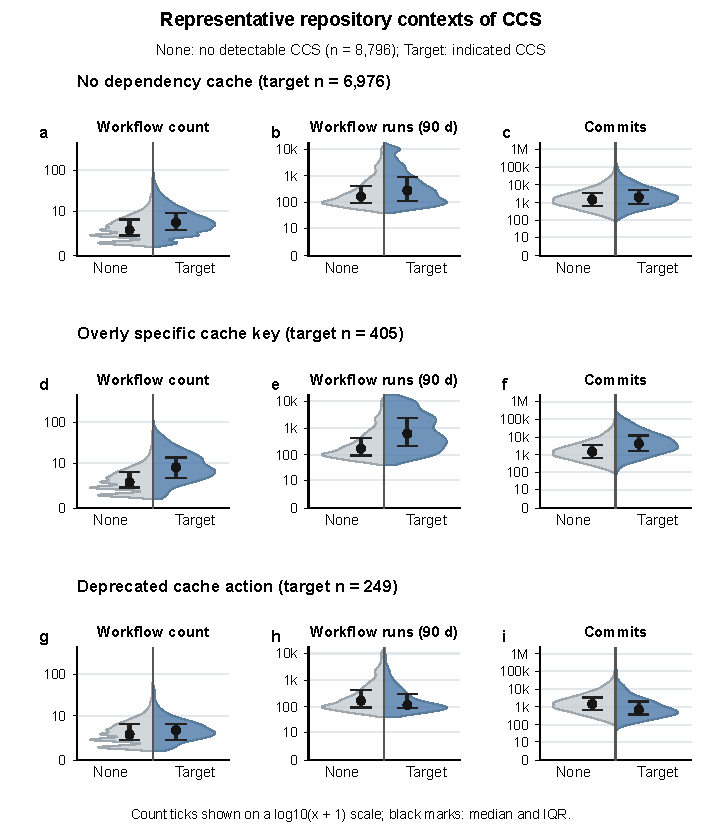
\includegraphics[width=\linewidth]{figures/rq1_representative_repository_contexts_split_violin_ccs.pdf}
\caption{Repository feature distributions for three representative CCS types.}
\label{fig:repository-feature-distribution}
\end{figure}

\paragraph{Workflow-role distribution.}
Table~\ref{tab:workflow-role-distribution} summarizes prevalence by the mutually exclusive workflow roles inferred from job names. Mixed and deploy workflows had the highest prevalence of any CCS, whereas analyze and sync workflows had the lowest. The complete cross-tabulation is retained in the replication data.

\begin{table}[htbp]\caption{Prevalence of selected detectable CCS by inferred workflow type}\label{tab:workflow-role-distribution}\centering\footnotesize
\begin{tabular}{lrrrrrr}\hline
Role & Workflows & Any CCS & S1 & S4 & S10 & S2\\\hline
Analyze & 3,497 & 4.78\% & 2.55\% & 1.46\% & 0.37\% & 0.06\% \\
Build & 21,466 & 31.14\% & 16.95\% & 5.83\% & 2.00\% & 7.45\% \\
Deploy & 2,699 & 31.27\% & 26.86\% & 2.63\% & 0.22\% & 1.78\% \\
Integration & 201 & 29.85\% & 17.41\% & 6.97\% & 3.98\% & 2.99\% \\
Lint & 3,636 & 21.04\% & 15.37\% & 3.33\% & 0.69\% & 0.36\% \\
Mixed & 17,523 & 34.31\% & 20.25\% & 9.64\% & 4.11\% & 4.97\% \\
Other & 46,358 & 13.35\% & 8.38\% & 2.65\% & 0.57\% & 1.91\% \\
Release & 5,838 & 17.39\% & 12.56\% & 1.88\% & 0.24\% & 2.79\% \\
Sync & 1,017 & 8.16\% & 6.88\% & 1.08\% & 0.20\% & 0.49\% \\
Test & 13,372 & 31.19\% & 19.07\% & 8.76\% & 3.63\% & 1.77\% \\
Update & 2,795 & 14.28\% & 10.95\% & 1.36\% & 0.11\% & 0.75\% \\\hline
\end{tabular}\par\smallskip\parbox{\linewidth}{\footnotesize\emph{Note.} S1: missing dependency cache; S4: missing fallback matching; S10: redundant cache update; S2: missing Docker layer cache. Rates use the workflow count in each row.}\end{table}

Mixed workflows combine several recognized tasks and therefore provide more opportunities for a cache-related finding within one file. Differences in dependency installation and Docker builds also contribute to the role-specific rates.

\paragraph{Repository-level exposure and within-repository concentration.} We distinguish repositories with at least one affected workflow from the fraction of affected workflows within a repository. The concentration table reports both measures by workflow-count group. Overall union measures are available in \texttt{rq1\_repository\_exposure.csv}. Repository exposure increased from 32.34\% among single-workflow repositories to 83.95\% among repositories with more than 20 workflows, while affected-workflow prevalence decreased from 32.34\% to 18.51\%. The denominators explain this contrast: a larger workflow collection offers more opportunities for at least one finding, even when most additional workflows contain no CCS.

\begin{table}[htbp]\caption{Repository and workflow prevalence by observed workflows per repository}\label{tab:repository-concentration}\centering\small\begin{tabular}{lrrrr}\hline
Workflows/repo. & Repositories & With CCS (\%) & Workflows & With CCS (\%)\\\hline
1 & 2,310 & 32.34\% & 2,310 & 32.34\% \\
2--3 & 5,827 & 46.37\% & 14,469 & 28.16\% \\
4--5 & 4,273 & 56.19\% & 18,946 & 25.36\% \\
6--10 & 4,395 & 61.23\% & 32,803 & 21.60\% \\
11--20 & 1,815 & 76.91\% & 25,671 & 20.24\% \\
$>20$ & 704 & 83.95\% & 24,203 & 18.51\% \\\hline
\end{tabular}\end{table}

\rqanswer{RQ1.1}{At least one CCS rule was triggered in 22.29\% of workflows and in a workflow from 54.48\% of repositories. \path{no_dependency_cache} was the most prevalent individual rule. Prevalence varied across repository languages, workflow roles, triggers, and repository characteristics. Python-primary repositories had the highest prevalence of workflows with any of the 11 CCS types, but their union prevalence excluding NDC was 9.00\%. Mixed and deployment workflows had the highest role-specific prevalence. Repositories with more workflows were more likely to contain a CCS finding, although a smaller share of their workflows was affected.}

\subsubsection{Multiplicity and Co-occurrence (RQ1.2)}

Across the 118,402 workflows with usable detector results, \path{no_fallback_cache} and \path{static_cache_key} co-occurred most often (1,596 workflows, 1.35\% of the corpus). This pair also had the largest Jaccard overlap among the frequent pairs (0.271). Selected pair counts and Jaccard indices are in Online Resource~1 (Table~S1). The complete 11-rule matrix is in \texttt{rq1\_cooccurrence.csv}.

Most affected workflows contained one CCS type (83.66\%). Four or more types occurred in 267 workflows (Table~\ref{tab:smell-multiplicity}).

\begin{table}[htbp]\caption{Distribution of CCS rule counts per workflow}\label{tab:smell-multiplicity}\centering\scriptsize\begin{tabular}{lrr}\hline
CCS types per workflow & Workflows & Share\\\hline
0 & 92,014 & 77.71\% \\
1 & 22,076 & 18.64\% \\
2 & 3,083 & 2.60\% \\
3 & 962 & 0.81\% \\
4 or more & 267 & 0.23\% \\\hline
\end{tabular}\end{table}

\rqanswer{RQ1.2}{Among affected workflows, 83.66\% triggered only one rule. The most frequent pair was \path{no_fallback_cache} and \path{static_cache_key} (1,596 workflows). This pair also had the highest Jaccard similarity among the frequent pairs (0.27).}


\subsection{Duration, Success, and Resource Use (RQ2)}

\paragraph{Common analysis sample.}

After detector screening, the RQ2 dataset contained 1,091,978 runs from 51,097 workflow versions in 14,695 repositories. Outcome screening retained 1,047,015 runs for success (50,460 versions and 14,632 repositories) and 1,089,617 runs for completed-run duration (50,985 versions and 14,690 repositories). Each unified model used the same outcome sample for every estimable CCS coefficient. Tables~\ref{tab:rq2-duration} and~\ref{tab:rq2-reliability} report the resulting associations. Figure~\ref{fig:rq2-unified-associations} summarizes the estimates and confidence intervals for both outcomes.

\paragraph{Model fit.}
Each primary model yielded 10 estimable CCS coefficients. Unreachable cache writes had no exposed version. The completed-run duration model had weighted $R^2=0.344$ and RMSE of 1.505 log seconds. The success LPM had weighted $R^2=0.060$ and mean squared error of 0.107. Fitted success values fell outside $[0,1]$ for 1.43\% of runs (1.30\% under version-balanced weights). The maximum VIF was 5.91 and the largest standardized condition number was 6.06 across the two models. Online Resource~2 reports full diagnostics and coefficient estimates.

\begin{figure}[tbp]
\centering
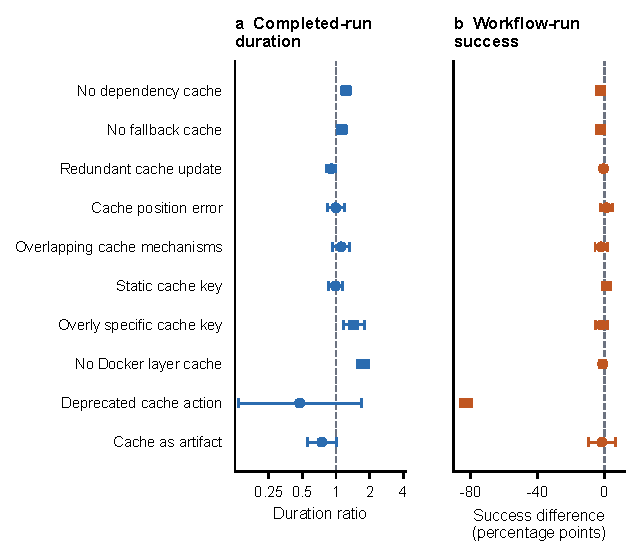
\includegraphics[width=\linewidth]{figures/rq2_adjusted_associations_forest.pdf}
\caption{Adjusted associations from the unified models: \textbf{a} completed-run duration ratios and \textbf{b} success-probability differences in percentage points. Bars show repository-clustered pointwise 95\% confidence intervals. Squares indicate BH-FDR $q<0.05$. Circles indicate other estimable coefficients. Dashed lines mark no association (ratio 1 or difference 0). Unreachable cache writes are not shown because their coefficient is not estimable.}
\label{fig:rq2-unified-associations}
\end{figure}

\subsubsection{Associations with Completed-Run Duration (RQ2.1)}

Four CCS types were associated with longer completed runs after BH correction (Table~\ref{tab:rq2-duration}). The adjusted difference ranged from 12.31\% for missing fallback matching to 74.70\% for missing Docker layer caching. Missing dependency caching and overly specific keys were associated with 23.06\% and 44.08\% longer duration, respectively. These associations are consistent with repeated acquisition or preparation of content when reuse is limited, although the observational models do not establish the underlying mechanism.

Redundant cache updates, deprecated cache actions, and caches used as artifacts had duration ratios below one, but none met the BH criterion. Short failed runs can reduce completed-run duration without improving execution, particularly when no exposed run succeeds. These estimates therefore provide insufficient evidence of a performance benefit. Cache placement errors, overlapping mechanisms, and static keys likewise showed no significant duration association after correction.

\begin{table}[tbp]
\centering\small
\caption{Adjusted associations with completed-run duration}
\label{tab:rq2-duration}
\begin{tabularx}{\linewidth}{@{}Yrrr@{}}
\hline
\textbf{CCS} & \textbf{Runs} & \textbf{Duration ratio [95\% CI]} & \textbf{$q$} \\
\hline
Missing dependency cache & 1,089,617 & \textbf{1.23 [1.13, 1.34]} & $2.09\times10^{-5}$ \\
Missing Docker layer cache & 1,089,617 & \textbf{1.75 [1.55, 1.97]} & $1.10\times10^{-18}$ \\
Deprecated cache action & 1,089,617 & 0.47 [0.13, 1.68] & 0.319 \\
Missing fallback matching & 1,089,617 & \textbf{1.12 [1.02, 1.23]} & 0.039 \\
Static cache key & 1,089,617 & 0.99 [0.86, 1.13] & 0.954 \\
Overly specific cache key & 1,089,617 & \textbf{1.44 [1.16, 1.79]} & 0.003 \\
Cache used as an artifact & 1,089,617 & 0.75 [0.55, 1.01] & 0.092 \\
Cache placement error & 1,089,617 & 0.99 [0.83, 1.19] & 0.954 \\
Unreachable cache write & 1,089,617 & Not estimable & -- \\
Redundant cache update & 1,089,617 & 0.91 [0.82, 1.00] & 0.091 \\
Overlapping mechanisms & 1,089,617 & 1.11 [0.93, 1.33] & 0.319 \\
\hline
\end{tabularx}
\par\smallskip
\parbox{\linewidth}{\footnotesize\emph{Note.} All coefficients come from one version-balanced model with a common sample and repository-clustered 95\% CIs. Bold estimates meet $q<0.05$. BH correction covers 10 estimable CCS coefficients. Unreachable writes have no exposed version. Full coefficients, SEs, raw $p$-values, and exposure counts are in Online Resource~2.}
\end{table}

\rqanswer{RQ2.1}{Four CCS types---\path{no_dependency_cache}, \path{no_fallback_cache}, \path{overly_specific_cache_key}, and \path{no_docker_layer_cache}---were associated with longer completed runs after adjustment for the other CCS types and controls, followed by BH correction. Their adjusted duration ratios ranged from 1.12 to 1.75.}

\subsubsection{Associations with Workflow-Run Success (RQ2.2)}

Three CCS types were associated with lower workflow-run success probability after BH correction (Table~\ref{tab:rq2-reliability}). Missing dependency caching and missing fallback matching were associated with decreases of 2.42 and 2.23 percentage points, respectively ($q<0.001$ and $q=0.031$). The other seven estimable CCS coefficients did not meet the corrected significance criterion. Run conclusions also reflect tests, infrastructure, and external services, so these associations do not identify which failures are attributable to caching.

Deprecated cache actions occurred in 33 versions across 22 repositories in the success sample, with 652 failed runs and no successful run. The LPM estimated an 82.52-percentage-point lower success probability (95\% CI: $-85.85$ to $-79.19$, $q<0.001$). This estimate uses the same clustered inference and BH family as the other CCS coefficients. Its magnitude and interval require caution because exposure is concentrated in relatively few repositories. Retirement of the legacy cache service offers a plausible explanation~\citep{gha_cache_action}, but individual failures would need to be checked against their logs.

\begin{table}[tbp]
\centering\small
\caption{Adjusted associations with workflow-run success}
\label{tab:rq2-reliability}
\begin{tabularx}{\linewidth}{@{}Yrrr@{}}
\hline
\textbf{CCS} & \textbf{Runs} & \shortstack{\textbf{Success difference}\\\textbf{(pp) [95\% CI]}} & \textbf{$q$} \\
\hline
Missing dependency cache & 1,047,015 & \textbf{-2.42 [-3.68, -1.15]} & $8.90\times10^{-4}$ \\
Missing Docker layer cache & 1,047,015 & -0.92 [-2.74, 0.90] & 0.538 \\
Deprecated cache action & 1,047,015 & \textbf{-82.52 [-85.85, -79.19]} & $<0.001$ \\
Missing fallback matching & 1,047,015 & \textbf{-2.23 [-3.90, -0.55]} & 0.031 \\
Static cache key & 1,047,015 & 1.32 [-1.38, 4.02] & 0.538 \\
Overly specific cache key & 1,047,015 & -1.70 [-5.45, 2.06] & 0.538 \\
Cache used as an artifact & 1,047,015 & -1.44 [-9.62, 6.74] & 0.731 \\
Cache placement error & 1,047,015 & 1.38 [-2.34, 5.11] & 0.584 \\
Unreachable cache write & 1,047,015 & Not estimable & -- \\
Redundant cache update & 1,047,015 & -0.47 [-2.47, 1.52] & 0.714 \\
Overlapping mechanisms & 1,047,015 & -1.76 [-5.55, 2.03] & 0.538 \\
\hline
\end{tabularx}
\par\smallskip
\parbox{\linewidth}{\footnotesize\emph{Note.} All coefficients come from one version-balanced LPM. Values are adjusted success-probability differences in percentage points (pp), with repository-clustered pointwise 95\% CIs. Bold estimates meet $q<0.05$. BH correction covers 10 estimable coefficients, including deprecated actions. Unreachable writes have no exposed version. Full coefficients and exposure counts are in Online Resource~2.}
\end{table}

\rqanswer{RQ2.2}{\path{no_dependency_cache}, \path{no_fallback_cache}, and \path{deprecated_cache_action} were significantly associated with lower workflow-run success probability in the unified LPM after BH correction. The corresponding adjusted differences were $-2.42$, $-2.23$, and $-82.52$ percentage points.}


\paragraph{Controls and sensitivity checks.}
The two models adjust jointly for workflow size, task, ecosystem, runner environment, event, and observation week. Online Resource~2 reports all coefficients and reference categories. The successful-run duration sensitivity analysis used 929,233 runs from 46,214 versions in 13,976 repositories. It is reported separately because restricting the sample to successful runs changes the outcome population.

\begingroup
\raggedbottom
\subsubsection{Observed VM Time and Estimated Runner Cost (RQ2.3)}

The historical comparison retained 166 change events from 88 repositories, covering 1,268 resource-complete successful runs and nine CCS types. Events may involve multiple types, so the type-specific counts in Table~\ref{tab:rq2-resource-cost} are not independent. We found no qualifying comparisons for deprecated cache actions or unreachable cache writes. Artifact-like cache use appeared in one repository.

Per-run VM-time and estimated-cost differences were positive for redundant updates, overly specific keys, and missing Docker layer caching. Their cost differences ranged from US\$0.0612 to US\$0.0950, with pointwise intervals above zero. These comparisons involved only four to six repositories per type. Missing dependency caching had a small positive cost difference, whereas missing fallback matching had a negative difference. Both intervals included zero. The negative differences for placement errors and artifact-like use do not establish resource savings from these configurations.

Complete monthly frequency records were available for 52 of the 88 repositories, covering 105 historical events. At the compared workflows' observed frequencies, redundant updates corresponded to US\$2.41 more per repository-month (95\% interval [0.31, 4.92]). The monthly equivalents were US\$1.42 for overly specific keys and US\$2.61 for missing Docker layer caching, each based on three repositories. These figures cover only compared workflows, not all workflow activity within a repository. Monthly coverage and weighting differ from the full per-run comparison, so changes in direction are not merely unit conversions.

Other workflow changes limit attribution: 107 events involved changed tasks or unresolved task comparability, and 53 had only one observation on at least one side. For example, a missing-dependency-cache introduction in \texttt{netatalk/netatalk} coincided with a macOS-to-Linux migration and changes to tool installation. Mean VM time fell from 295.0 to 109.3 seconds, while estimated cost fell from US\$0.346 to US\$0.032. Such changes can outweigh cache-related differences, so negative estimates should not be interpreted as benefits of CCS.

\begin{table}[H]
\centering
\caption{Historical within-workflow differences in runner time and estimated runner cost}
\label{tab:rq2-resource-cost}
\begingroup
\small
\setlength{\tabcolsep}{3pt}
\renewcommand{\arraystretch}{1.15}
\begin{tabularx}{\linewidth}{@{}Yrrrr@{}}
\hline\noalign{\smallskip}
\textbf{CCS} & \shortstack{\textbf{Events/}\\\textbf{repos.}} & \shortstack{\textbf{$\Delta$ VM}\\\textbf{min/run}} & \shortstack{\textbf{$\Delta$ cost (US\$)/run}\\\textbf{[95\% interval]}} & \shortstack{\textbf{$\Delta$ US\$/month}\\\textbf{(repos.)}} \\
\noalign{\smallskip}\hline\noalign{\smallskip}
Missing dependency cache & 106/59 & +0.29 & \shortstack{+0.0086\\{\scriptsize [-0.0291, +0.0463]}} & -0.61 (33) \\[3pt]
Missing fallback matching & 46/24 & +2.70 & \shortstack{-0.0165\\{\scriptsize [-0.1003, +0.0607]}} & -2.85 (16) \\[3pt]
Redundant cache update & 7/6 & +3.06 & \shortstack{+0.0875\\{\scriptsize [+0.0023, +0.2172]}} & +2.41 (6) \\[3pt]
Cache placement error & 2/2 & -13.85 & \shortstack{-0.1353\\{\scriptsize [-0.3047, +0.0340]}} & -1.82 (2) \\[3pt]
Overlapping mechanisms & 8/6 & +1.01 & \shortstack{+0.0092\\{\scriptsize [-0.0067, +0.0264]}} & +0.05 (4) \\[3pt]
Static cache key & 17/6 & +2.83 & \shortstack{+0.0359\\{\scriptsize [-0.0043, +0.1055]}} & +8.08 (3) \\[3pt]
Overly specific cache key & 4/4 & +7.20 & \shortstack{+0.0612\\{\scriptsize [+0.0107, +0.1225]}} & +1.42 (3) \\[3pt]
Missing Docker layer cache & 6/4 & +11.66 & \shortstack{+0.0950\\{\scriptsize [+0.0264, +0.1807]}} & +2.61 (3) \\[3pt]
Deprecated cache action & 0/0 & -- & -- & -- \\[3pt]
Unreachable cache write & 0/0 & -- & -- & -- \\[3pt]
Cache used as an artifact & 1/1 & -11.33 & -0.0760 & -- \\[3pt]
\noalign{\smallskip}\hline
\end{tabularx}
\parbox{0.96\linewidth}{\footnotesize\emph{Note.} Differences are detected minus undetected for successful runs. Per-run estimates average events within repositories, then weight repositories equally. Intervals are pointwise repository-bootstrap intervals, without multiple-testing adjustment. No interval is reported for a single repository. Monthly equivalents use each compared workflow's actual April--May 2026 run counts. Parentheses give frequency-covered repository counts. Missing comparisons are shown as --, not zero. Amounts use the fixed historical reference model in Section~\ref{sec:analysis-methods} and are not actual bills or causal repair savings.}
\endgroup
\end{table}

\rqanswer{RQ2.3}{Historical CCS changes coincided with differences in VM time and estimated runner cost. Redundant updates, overly specific keys, and missing Docker layer caching had positive per-run differences in both measures, based on four to six repositories each. Concurrent workflow changes and limited coverage prevent interpreting these differences as costs caused by CCS.}
\endgroup

\section{Discussion}
\label{sec:discussion}

\subsection{Synthesis of Findings}

CCS appeared in a minority of workflows but in more than half of the studied repositories. Their prevalence varied with repository language, workflow triggers and roles, and repository activity. Cache configuration review should therefore consider both the workflow's dependency operations and its role within the repository.

The unified outcome models identified four CCS types associated with longer completed runs and three associated with lower success probability after covariate adjustment and BH correction. Missing dependency caching and missing fallback matching were associated with both outcomes. Overly specific keys and missing Docker layer caching were associated with duration, while deprecated actions showed the largest success-probability difference. The separate descriptive resource comparisons provide additional context but use different, CCS-specific eligible samples.

Several cache mechanisms could explain the duration findings. Missing dependency caches or fallback keys can lead to repeated downloads, overly specific keys can limit reuse, and missing Docker layer caching can require repeated image-layer preparation. Run conclusions also reflect failures in tests, infrastructure, and external services. Direct measurements of cache behavior and configuration changes are needed to determine which mechanisms account for the observed associations.

\subsection{Relation to Prior Evidence}

Prior work has examined CI build duration, pipeline refactoring, and cache-related configuration problems~\citep{ghaleb2019empirical,ghaleb2022studying,zampetti2021ci,urdih2026cache}. Ghaleb et al. found that build-time improvements after caching adoption varied across Travis CI projects~\citep{ghaleb2026cachingreality}, highlighting the role of ongoing maintenance and cache-operation overhead. Our study extends this evidence to GitHub Actions by relating specific CCS types to workflow runs aligned with the analyzed configuration versions. The prevalence of missing dependency caching and fallback matching is also consistent with earlier findings that dependency acquisition and cache reuse are recurring optimization concerns~\citep{gallaba2022caching,bouzenia2024resource,hasan2026caching}.

We apply the job-level VM-time and fixed-reference-pricing approach of \citet{bouzenia2024resource} to samples eligible for each CCS rule. While their study characterized resource use across GitHub Actions workloads, we compare workflow versions with and without each detectable CCS type. The detection rules thus connect resource-use comparisons to specific configurations that practitioners can inspect.

\subsection{Tool Support for Workflow Review}
\label{subsec:tool-support}

We packaged the detector as \textit{Workflow Cache Inspector}, a tool with a web interface for reviewing GitHub Actions workflows (Fig.~\ref{fig:tool-ui}). Users enter a repository name in \texttt{owner/repository} format and a workflow file path. The tool scans the specified file on the default branch and returns a report covering the 11 CCS types. The report summarizes findings by type and links to the source workflow. Individual findings identify the affected job and provide an explanation and a suggested fix. Users can also download the report in JSON format.

The illustrated scan of \texttt{pallets/flask} and \path{.github/workflows/tests.yaml} reports one \path{no_fallback_cache} finding in the \texttt{typing} job. It explains that the cache lacks an effective fallback when the primary key misses and suggests adding \texttt{restore-keys} with broader prefixes. This connects a detected pattern to a change that developers can review against their intended cache policy. The tool retains the detector's static-analysis scope: a scan with no findings does not establish cache correctness, and suggested changes require compatibility checks and evaluation through comparable workflow runs.

\begin{figure}[p]
\centering
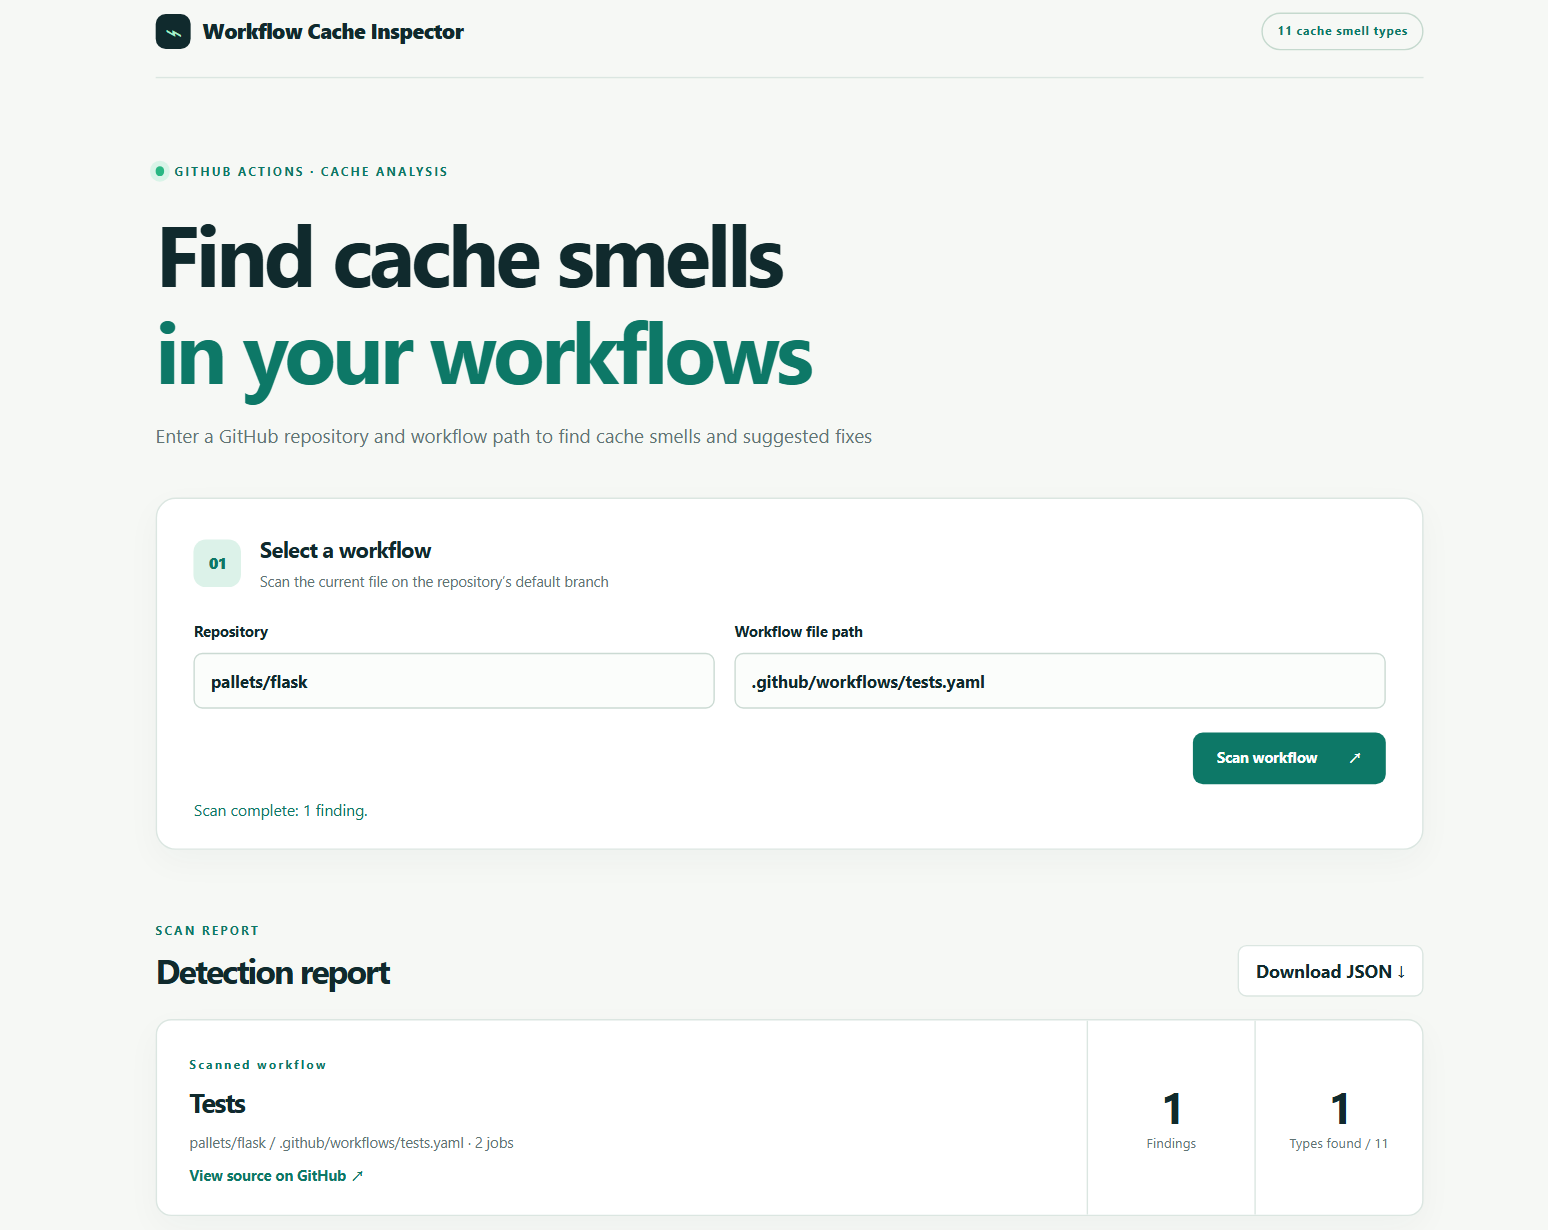
\includegraphics[width=\linewidth,height=0.43\textheight,keepaspectratio]{figures/tool_ui_1.png}
\par\smallskip
{\small (a) Repository and workflow selection.}
\par\medskip
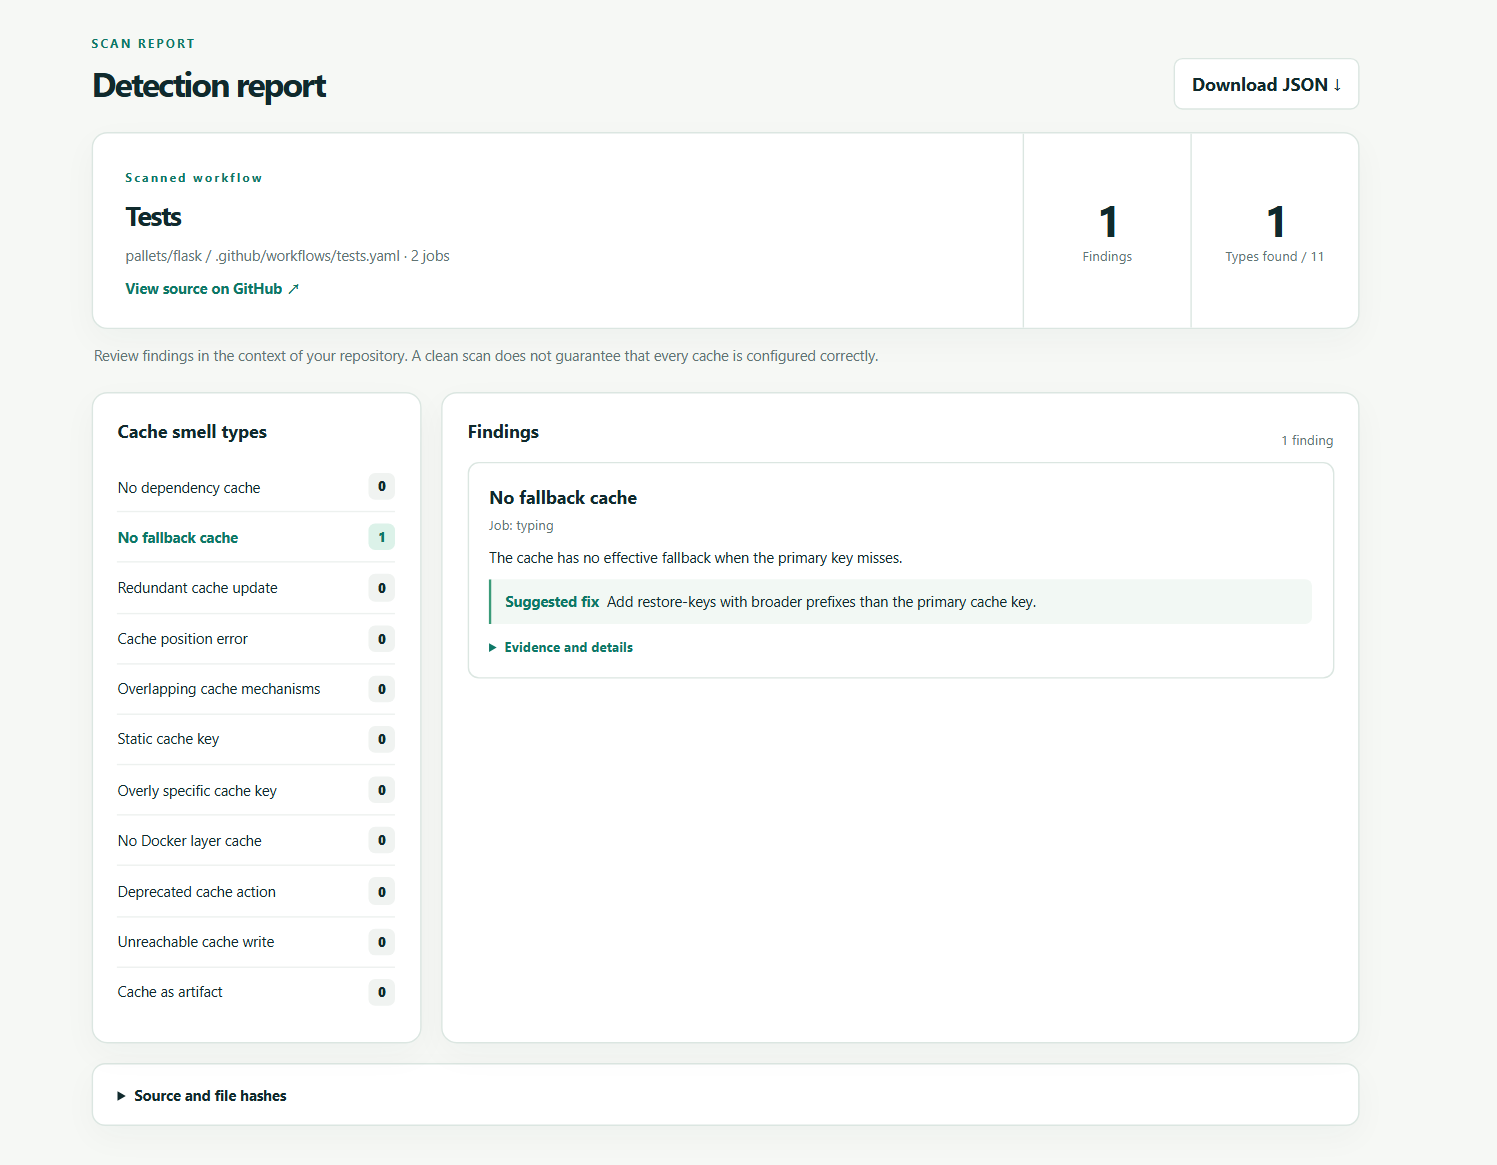
\includegraphics[width=\linewidth,height=0.43\textheight,keepaspectratio]{figures/tool_ui_2.png}
\par\smallskip
{\small (b) Findings by CCS type and suggested fix.}
\caption{Workflow Cache Inspector: workflow input and detection report for the illustrated \texttt{pallets/flask} scan.}
\label{fig:tool-ui}
\end{figure}
\FloatBarrier

\subsection{Implications}

\paragraph{Review the cache lifecycle before adding more caching.}
Missing dependency caching was the most prevalent CCS, making supported installation steps a practical starting point for review. Practitioners can then follow the cache data flow: identify reusable content, restore it before consumption, and save it after production. Because missing fallback matching co-occurred with static keys and redundant updates, key changes should be reviewed together with restore and save policies. Broader fallback keys may improve reuse for a dependency-download store when the restored content remains compatible with installation. Build outputs tied to exact inputs require a different policy. Reviewing these relationships together helps translate co-occurring findings into a coherent configuration change.

\paragraph{Evaluate changes using feedback time and resource use.}
The four duration-associated types identify configurations worth reviewing. Their ratios come from a common adjusted model but cannot rank expected repair benefits. Practitioners can evaluate a change through repeated runs of the same task, measuring cold-cache and warm-cache behavior before and after the change. Relevant measurements include restore and save time, dependency-installation time, workflow duration, and aggregate job time. The historical comparisons illustrate why elapsed time alone is insufficient: operating-system choice and job structure also affect estimated cost. Reducing feedback delay may leave aggregate runner use unchanged, while successful runs can still perform avoidable work~\citep{bouzenia2024resource,ghaleb2026cachingreality}.

\paragraph{Make lint findings explain the relevant configuration relationship.}
Lint tools should explain the configuration relationship behind each warning. A placement warning should identify the cache, the inputs needed to resolve its key, and the consumer that ran before restoration. A redundant-update warning should identify competing jobs, expanded keys, and the missing coordination. This evidence helps developers assess findings when YAML does not reveal the intended cache policy. For opaque actions, reports can identify the internal behavior that needs inspection. Such explanations follow the detection-and-repair presentation used by configuration-smell tools~\citep{zhang2022buildsonic,urdih2026cache}.

\paragraph{Separate mechanical migrations from changes to reuse policy.}
Deprecated cache-action versions have an explicit support boundary and are candidates for targeted migration after compatibility checks. Changes to fallback keys, shared keys, or overlapping mechanisms require closer review because they alter content reuse or responsibility for cache preparation. Tools should explain these changes and check paths, platform dimensions, and dependencies before proposing a patch. Several rules have few manually confirmed positive cases, making developer feedback especially useful for evaluating suggestions. As in prior smell-repair work, evaluation should assess behavior preservation, developer acceptance, and duration effects separately~\citep{zhang2022buildsonic}.

\paragraph{Study which detected configurations cause avoidable work.}
Researchers can connect static findings to cache hits, transferred bytes, installation work, and save attempts to establish when a detected pattern leads to avoidable work. Within-workflow comparisons can help isolate configuration changes when task, runner, and dependency versions remain stable. Repeated runs should separate initial cache population from subsequent reuse. Evaluation on annotated repositories excluded from rule development would test whether detection accuracy generalizes beyond the development cases. Cross-platform studies can examine the shared concerns while specifying platform-dependent semantics for action versions, key matching, and setup-action caches~\citep{urdih2026cache,hasan2026caching}.

\section{Threats to Validity}
\label{sec:threats}

\paragraph{Construct validity.}
Static rules approximate configuration concerns and may miss behavior inside scripts, reusable workflows, or custom actions. Some CCS types have few positive reference workflows, limiting the evidence for their detection accuracy. Repository language and job-name roles are approximations of workflow context. Run-to-version linkage uses workflow identities and last-change intervals without checking YAML at every run's \texttt{head\_sha}. Incorrect boundaries could misclassify CCS presence. Duration and run conclusions include work and failures unrelated to caching. Estimated cost uses a fixed reference model whose coverage depends on operating-system recognition, job-level rounding, and job availability.

\paragraph{Internal validity.}
Measured controls account for observed workload and environment differences, and repository-clustered uncertainty accounts for dependent observations. Unmeasured task complexity, runner conditions, and project practices may still be associated with CCS. The duration model leaves substantial variation unexplained. The LPM assumes additive linear probability differences and produced fitted values outside $[0,1]$ for 1.43\% of runs. Clustered inference for deprecated actions also warrants caution because only 22 repositories were exposed. Repository-feature contrasts and resource comparisons do not adjust for confounding. The results therefore describe associations and observed differences. Controlled comparisons are needed to estimate repair benefits.

\paragraph{External and temporal validity.}
The sample consists of non-forked public GitHub repositories selected using star, commit, and run thresholds. Findings may differ for private or less active projects and other CI/CD platforms. RQ2.1 and RQ2.2 cover 30 days of default-branch runs. RQ2.3 uses available historical changes, but resource archives are incomplete and comparisons retain only successful runs. Monthly equivalents assume historical differences transfer to observed April--May 2026 frequencies. Cache services, action versions, and runner offerings change over time, so replication must use the documented cutoff and detector snapshot. The cost model supports comparisons within the study and does not estimate current charges.

\section{Conclusion}
\label{sec:conclusion}

We defined 11 cache configuration smell types for GitHub Actions and evaluated a static detector against manually reviewed workflows. At least one type appeared in 22.29\% of workflows and in workflows from 54.48\% of repositories. Missing dependency caching was the most prevalent type, and occurrence patterns varied with workflow tasks and repository activity.

Four types were associated with longer completed runs after covariate adjustment and multiple-testing correction. Missing dependency caching, missing fallback matching, and deprecated cache actions were associated with lower success probability. Separate descriptive analyses showed differences in runner time and estimated cost. These findings identify cache configuration relationships worth reviewing and motivate repair evaluations based on repeated, comparable workflow runs.

\bibliographystyle{spbasic}
\bibliography{references}

\end{document}
